\documentclass[10pt,a4paper]{ctexart}
\usepackage{geometry}
\geometry{a4paper, margin=2.3cm}
\usepackage{booktabs}
\usepackage{graphicx}
\usepackage{amsmath}
\usepackage{amssymb}
\usepackage{longtable}
\usepackage{caption}
\usepackage{setspace}
\usepackage{enumitem}
\usepackage{xcolor}
\usepackage{hyperref}
\usepackage{float}
\usepackage{multirow}
\usepackage{array}
\usepackage{subcaption}

% 全局设置
\setlength{\parindent}{2em}
\linespread{1.25}
\hypersetup{colorlinks=true, linkcolor=blue, citecolor=blue, urlcolor=blue}

\title{\textbf{综合收益率(Shareholder Yield)策略:\\极端值剔除必要性论证与指数增强研究}}
\author{}
\date{\today}

\begin{document}

\maketitle

\begin{abstract}
在港股量化选股策略中，综合收益率（Shareholder Yield = 股息收益率 + 回购收益率）是一个兼具价值与质量双重属性的强大因子。然而，一个关键的方法论问题长期被忽视：\textbf{极端高收益率的股票究竟是Alpha信号还是价值陷阱？}

本报告通过系统的实证研究，以恒生综合指数（HSCI）为股票池、2012-2025年为回测区间，从七个维度——策略绩效对比、Fama-French三因子Alpha分析、市值-SY双重排序、极端值个股画像、FF3因子中性化、HSICS行业中性化、以及指数增强视角——论证了\textbf{极端值剔除是Shareholder Yield策略的"必选项"而非"可选项"}。核心发现如下：

\begin{enumerate}[label=(\arabic*)]
    \item \textbf{极端值剔除的边际贡献极大}：仅剔除得分前10\%的极端值，策略年化收益从5.78\%跃升至14.06\%，夏普比率从0.19升至0.63，FF3月度Alpha从-0.05\%（不显著）升至0.96\%（$t=5.40$, $p<0.001$）。
    \item \textbf{极端值是"小盘价值陷阱"}：被剔除的极端值股票平均市值仅处于全体股票的30分位数，78.7\%集中在市值后半段。其后续月均收益（0.44\%）显著低于正常高SY股票（0.60\%），年化差距约2\%。
    \item \textbf{负向预测以地产股为主}：最差的30只极端SY股票平均月收益为-5.17\%，包括中国奥园（-16.86\%/月）、时代中国控股（-13.93\%/月）等，97\%低于极端组中位市值。
    \item \textbf{行业中性化降低Alpha}：FF3价值(BM)中性化使策略C的IR从0.66降至0.40（-39\%），HSICS行业中性化使策略B的IR从1.11降至0.94（-15\%）。SY因子承载的是价值溢价+股东回报溢价，中性化等于剥离Alpha来源。
    \item \textbf{所有中性化方法均不推荐}：市值中性化几乎无影响(IR降0.04)，BM中性化严重破坏(IR降0.27)，行业+市值中性化介于两者之间。原始策略B(IR=1.11,月胜率64.4\%)和策略C(Sharpe=0.70,回撤-27.69\%)已是接近最优配置。
\end{enumerate}

\textbf{核心结论}：极端值剔除不是统计上的"数据清洁"，而是一个\textbf{基本面质量过滤器}——它系统性地移除了因股价暴跌导致收益率虚高的小市值困境公司。叠加低波动过滤后，策略C在保留显著Alpha（FF3月度0.71\%, $t=6.06$）的同时将最大回撤控制在-27.69\%（HSI同期为-55.34\%），可作为指数增强型策略进行配置。\textbf{不推荐对SY因子进行任何形式的中性化处理}。
\end{abstract}

% ================================================================
\section{研究背景与动机}
% ================================================================

\subsection{Shareholder Yield因子的理论基础}

在成熟资本市场中，上市公司通过两种主要方式向股东返还现金：\textbf{现金分红}和\textbf{股份回购}。传统的红利策略仅关注股息率，忽略了回购这一日益重要的股东回报渠道。尤其在港股市场，以腾讯、汇丰、友邦为代表的蓝筹公司在过去十年间进行了大规模的股份回购，其股东回报力度远超单纯的股息支付。

综合收益率（Shareholder Yield, SY）将两者统一度量：
\begin{equation}
\text{ShareholderYield}_i = \underbrace{\frac{\frac{1}{36}\sum_{t=1}^{36} (P_{i,t} \times DY_{i,t})}{P_{i,\text{current}}}}_{\text{股息收益率}} + \underbrace{\frac{\text{Buyback}_{i,[0,-35]} / 3}{\text{MarketCap}_{i,\text{current}}}}_{\text{回购收益率}}
\end{equation}

该因子的经济学含义是：股东通过分红和回购，每年能从公司市值中获得的总现金回报比例。

\subsection{核心研究问题}

在构建SY策略的过程中，一个关键的实证问题浮现：\textbf{因子得分最高的股票是否就是最好的投资标的？}

直觉上，高SY意味着高股东回报，应当对应更高的预期收益。然而，SY的分子（股息+回购）和分母（市值）都受市场波动影响——当股价暴跌时，即便分红和回购不变，SY也会机械性上升。这种"分母效应"可能使SY因子沦为"价值陷阱"的探测器：不是因为它发现了高回报的好公司，而是因为它标记了股价腰斩的困境公司。

因此，本报告围绕以下核心问题展开：
\begin{enumerate}[label=(\arabic*)]
    \item 极端高SY值是否系统性地来自小市值困境公司？
    \item 剔除极端值对策略绩效的影响有多大？
    \item 剔除的极端值股票后续表现如何？它们有什么共同特征？
    \item 行业中性化是否改善策略表现？
    \item 不同的风险过滤器（低波 vs. FCFF）哪个更优？
\end{enumerate}

% ================================================================
\section{数据与方法}
% ================================================================

\subsection{数据来源}

所有数据来自RiceQuant量化平台API，覆盖香港市场：

\begin{table}[htbp]
\centering
\caption{核心数据文件}
\begin{tabular}{lll}
\toprule
\textbf{文件} & \textbf{内容} & \textbf{频率} \\
\midrule
hk\_price.csv & 复权收盘价、成交额 & 日频 \\
hk\_dividendyield.h5 & 股息率（D/P） & 月频 \\
hk\_shares.h5 & 总股本 & 月频 \\
HSCI.csv & 恒生综合指数成分股 & 月频 \\
em\_buyback\_filtered.csv & 上市公司回购记录 & 日频 \\
hk\_ff3\_factors.csv & 香港Fama-French三因子 & 月频 \\
hk\_fcff.csv & 自由现金流（FCFF） & 年频 \\
HSI\_index.csv & 恒生指数（akshare爬取） & 日频 \\
hk\_stock\_connect\_high\_div.csv & 港股通高股息指数（CSI 930914） & 日频 \\
\bottomrule
\end{tabular}
\end{table}

\subsection{因子构建流程}

每个月底，执行以下计算流水线：

\textbf{第一步：基础池与流动性过滤。} 以HSCI成分股为基础池，剔除近3个月日均成交额（ADTV）或总市值处于市场后20\%的尾部股票。

\textbf{第二步：股东回报筛选。} 要求标的在过去36个月内存在分红记录（任意月份股息率>0）或回购记录（累计回购金额>0）。

\textbf{第三步：综合收益率计算。} 按公式(1)分别计算股息收益率和回购收益率，加总得到SY得分。

\textbf{第四步：极端值处理（核心差异点）。} 本报告对比了多种处理方式（详见策略设计）。

\textbf{第五步：持仓精选。} 按处理后的得分排序，取前20\%进入备选池，再根据风险过滤器（低波/FCFF）精选10-20只最终持仓。

\subsection{回测设置}

\begin{itemize}
    \item \textbf{回测区间}：2012年1月至2025年9月（共165个月）
    \item \textbf{调仓频率}：季度调仓（每3个月）
    \item \textbf{权重方案}：等权（Equal Weight）和受限市值加权（Cap Weight，单股上限10\%）
    \item \textbf{基准指数}：恒生指数（HSI）、港股通高股息指数（CSI 930914）
\end{itemize}

% ================================================================
\section{策略设计}
% ================================================================

为系统性地回答研究问题，我们设计了四种策略变体，通过控制变量法逐一检验每个处理步骤的边际贡献：

\begin{table}[htbp]
\centering
\caption{四种策略变体设计}
\begin{tabular}{lp{2.5cm}p{2.2cm}p{2.2cm}p{2.2cm}}
\toprule
\textbf{策略} & \textbf{极端值剔除} & \textbf{风险过滤器} & \textbf{持仓选择} & \textbf{研究目的} \\
\midrule
A: 纯SY无剔除 & 无 & 无 & SY得分前20只 & 基准：展示未处理SY的表现 \\
B: SY+剔除极端 & 剔除前10\% & 无 & SY得分前20只 & 检验极端值剔除的边际贡献 \\
C: SY+剔除+低波 & 剔除前10\% & 低波动率 & 前20\%SY中波动率最低20只 & 检验低波过滤的增量效果 \\
D: SY+剔除+FCFF & 剔除前10\% & FCFF>0 & 前20\%SY中FCFF>0取前20只 & 对比FCFF与低波过滤 \\
\bottomrule
\end{tabular}
\end{table}

\subsection{极端值剔除的操作定义}

对于每月横截面数据：
\begin{equation}
\text{cutoff}_t = Q_{0.90}(\text{score}_{i,t}, \; i \in \text{universe}_t)
\end{equation}

将SY得分>$Q_{0.90}$的股票标记为"极端组"，在策略B/C/D中予以剔除。

\subsection{行业中性化处理}

为检验行业偏差的影响，我们使用两种粒度的行业分类进行对比实验：

\textbf{粗略行业分类（代码区间法）}——基于香港股票代码的历史分配规律，将股票映射到16个行业组：
\begin{itemize}
    \item 00001-00099: 综合企业（最早期上市的综合型公司）
    \item 00100-00499: 地产建筑业
    \item 00500-00699: 非必需性消费
    \item 00700-00799: 工业
    \item 00800-00999: 非必需性消费
    \item 01000-01299: 非必需性消费
    \item 01300-01399: 金融业
    \item 01400-01899: 工业
    \item 01900-01999: 金融业
    \item 02000-02199: 必需性消费
    \item 02200-02899: 非必需性消费
    \item 02900-02999: 必需性消费
    \item 03000-03699: 工业
    \item 03700-03799: 非必需性消费
    \item 03800-03899: 原材料业
    \item 03900-03999: 地产建筑业
    \item 04000-05999: 工业
    \item 06000-06199: 金融业（银行）
    \item 06200-06299: 非必需性消费
    \item 06300-06399: 工业
    \item 06400-06599: 资讯科技业
    \item 06600-06699: 必需性消费
    \item 06700-06999: 地产建筑业
    \item 07000-07999: 资讯科技业
    \item 08000-08999: 非必需性消费
    \item 09000-09999: 工业
\end{itemize}

\textbf{精确行业分类（HSICS系统）}——基于恒生指数公司官方发布的HSICS（Hang Seng Industry Classification System），见附录PDF。该分类包含12个行业、31个业务类别和112个业务子类别，是香港股票市场最权威的行业分类标准。个股映射采用akshere验证数据结合代码区间辅助推断（详见§9）。

两种分类系统均用于行业中性化（行业内Z-score标准化），公式为：
\begin{equation}
\text{SY}_{\text{neutral},i} = \frac{\text{SY}_{\text{raw},i} - \bar{\text{SY}}_{\text{industry}}}{\sigma_{\text{SY},\text{industry}}}
\end{equation}

% ================================================================
\section{核心实证结果}
% ================================================================

\subsection{策略绩效全景对比}

\begin{table}[htbp]
\centering
\caption{六种策略/基准的绩效对比（等权配置，2012-2025）}
\begin{tabular}{lccccc}
\toprule
\textbf{策略} & \textbf{年化收益} & \textbf{年化波动} & \textbf{夏普比率} & \textbf{最大回撤} & \textbf{累计收益} \\
\midrule
A: 无剔除 & 5.78\% & 30.25\% & 0.19 & -74.49\% & 1.26$\times$ \\
B: 仅剔除 & \textbf{14.06\%} & 22.26\% & 0.63 & -35.19\% & 4.95$\times$ \\
C: 剔除+低波 & 11.40\% & \textbf{16.24\%} & \textbf{0.70} & \textbf{-27.69\%} & 3.99$\times$ \\
D: 剔除+FCFF & 13.45\% & 21.64\% & 0.62 & -36.26\% & 4.64$\times$ \\
\hline
HSI基准 & 3.49\% & 20.05\% & 0.17 & -55.34\% & 1.21$\times$ \\
港股通高股息 & 9.05\% & 24.76\% & 0.37 & -50.94\% & 2.34$\times$ \\
\bottomrule
\end{tabular}
\end{table}

\begin{figure}[H]
\centering
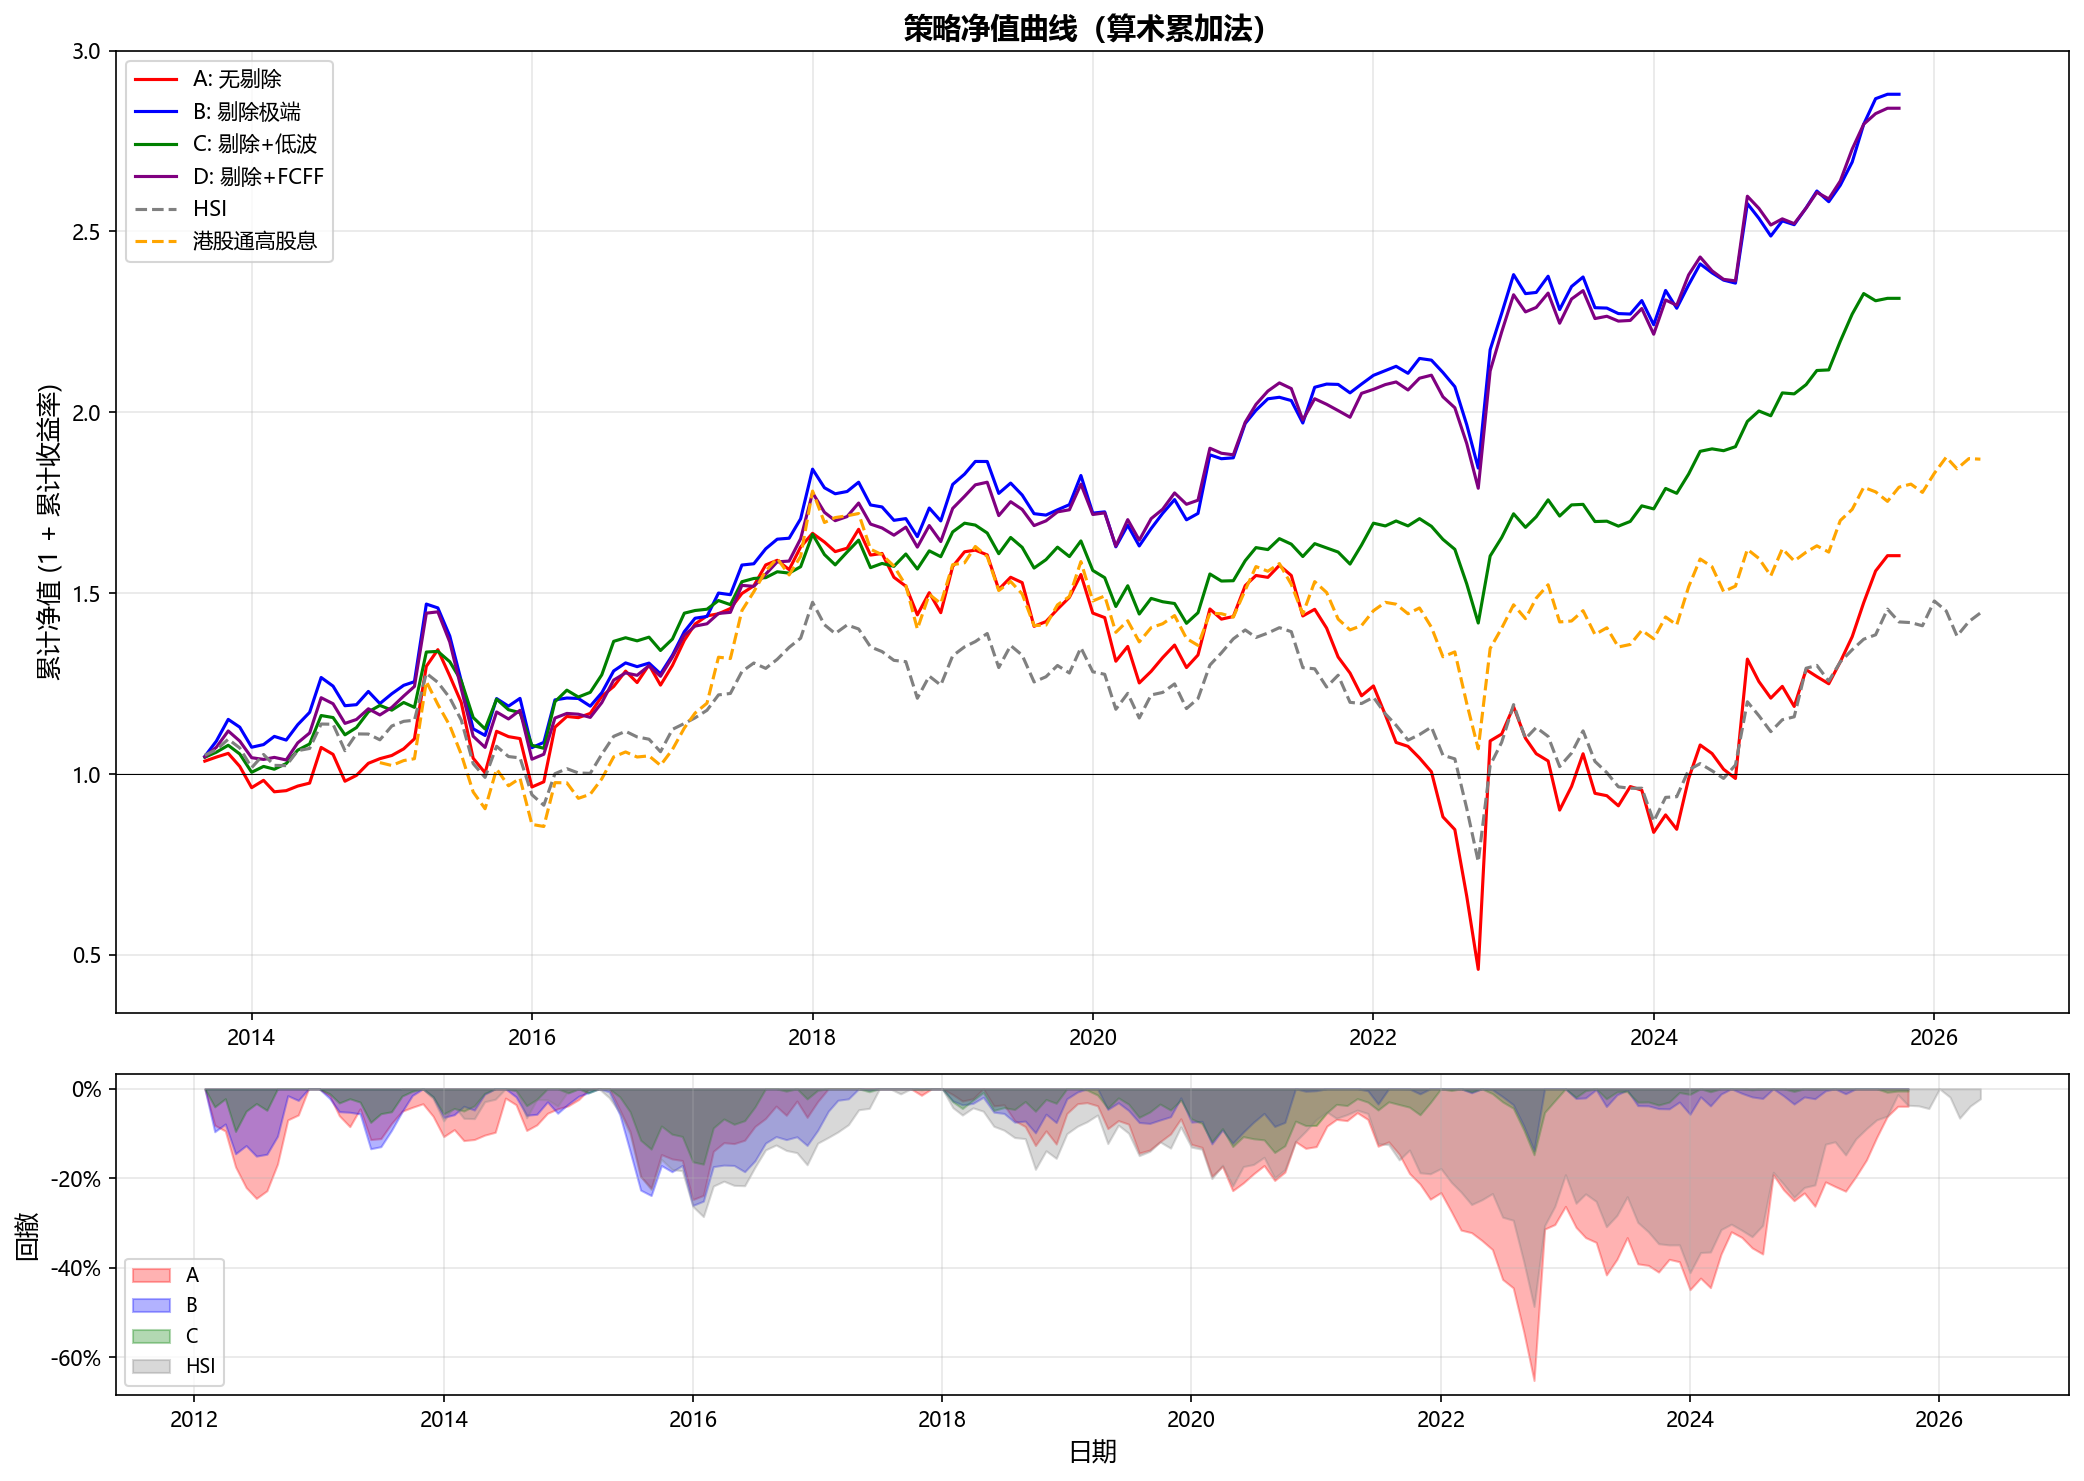
\includegraphics[width=0.92\textwidth]{../pict/v4_plot_01.png}
\caption{全部策略与基准的累计净值曲线（等权配置）}
\label{fig:cumulative}
\end{figure}

\textbf{核心发现}：从策略A到策略B的跃迁——仅添加一个极端值剔除步骤——年化收益提升8.28个百分点，夏普比率从0.19$\rightarrow$0.63（+230\%），最大回撤从-74.49\%$\rightarrow$-35.19\%（缩小53\%）。这一单一处理步骤的边际贡献远超任何其他优化。

\subsection{市值加权的稳健性检验}

\begin{table}[htbp]
\centering
\caption{受限市值加权（单股上限10\%）绩效对比}
\begin{tabular}{lccccc}
\toprule
\textbf{策略} & \textbf{年化收益} & \textbf{年化波动} & \textbf{夏普比率} & \textbf{最大回撤} & \textbf{累计收益} \\
\midrule
B: 仅剔除（CW） & \textbf{15.00\%} & 21.30\% & \textbf{0.70} & -35.67\% & 5.79$\times$ \\
C: 剔除+低波（CW） & 11.79\% & \textbf{16.88\%} & \textbf{0.70} & \textbf{-31.79\%} & 4.15$\times$ \\
\bottomrule
\end{tabular}
\end{table}

市值加权下结论一致：策略B收益更高（+15\%），策略C风险更低（波动仅16.88\%）。

\subsection{Fama-French三因子Alpha分析}

这是最关键的统计检验。如果极端值剔除仅仅是"数据清洁"，那么剔除前后的FF3 Alpha不应有本质差异。如果alpha发生剧变，说明剔除的不是噪声而是系统性偏差。

\begin{table}[htbp]
\centering
\caption{FF3 Alpha回归结果（Newey-West HAC, $k=3$）}
\begin{tabular}{lccccc}
\toprule
\textbf{策略} & \textbf{月度$\alpha$ (\%)} & \textbf{$t_{\alpha}$} & \textbf{p值} & \textbf{市场$\beta$} & \textbf{$R^2$} \\
\midrule
A: 无剔除 & -0.048 & -0.18 & 0.854 & 1.385 & 0.804 \\
B: 仅剔除 & \textbf{0.957***} & \textbf{5.40} & $<0.001$ & 1.067 & 0.889 \\
C: 剔除+低波 & \textbf{0.693***} & \textbf{5.36} & $<0.001$ & 0.739 & 0.868 \\
D: 剔除+FCFF & \textbf{0.909***} & \textbf{5.50} & $<0.001$ & 1.047 & 0.902 \\
\hline
HSI基准 & -0.050 & -0.45 & 0.653 & 0.990 & 0.948 \\
港股通高股息 & 0.345** & 2.30 & 0.022 & 1.199 & 0.905 \\
\bottomrule
\end{tabular}
\end{table}

\begin{figure}[H]
\centering
\begin{subfigure}{0.48\textwidth}
    \centering
    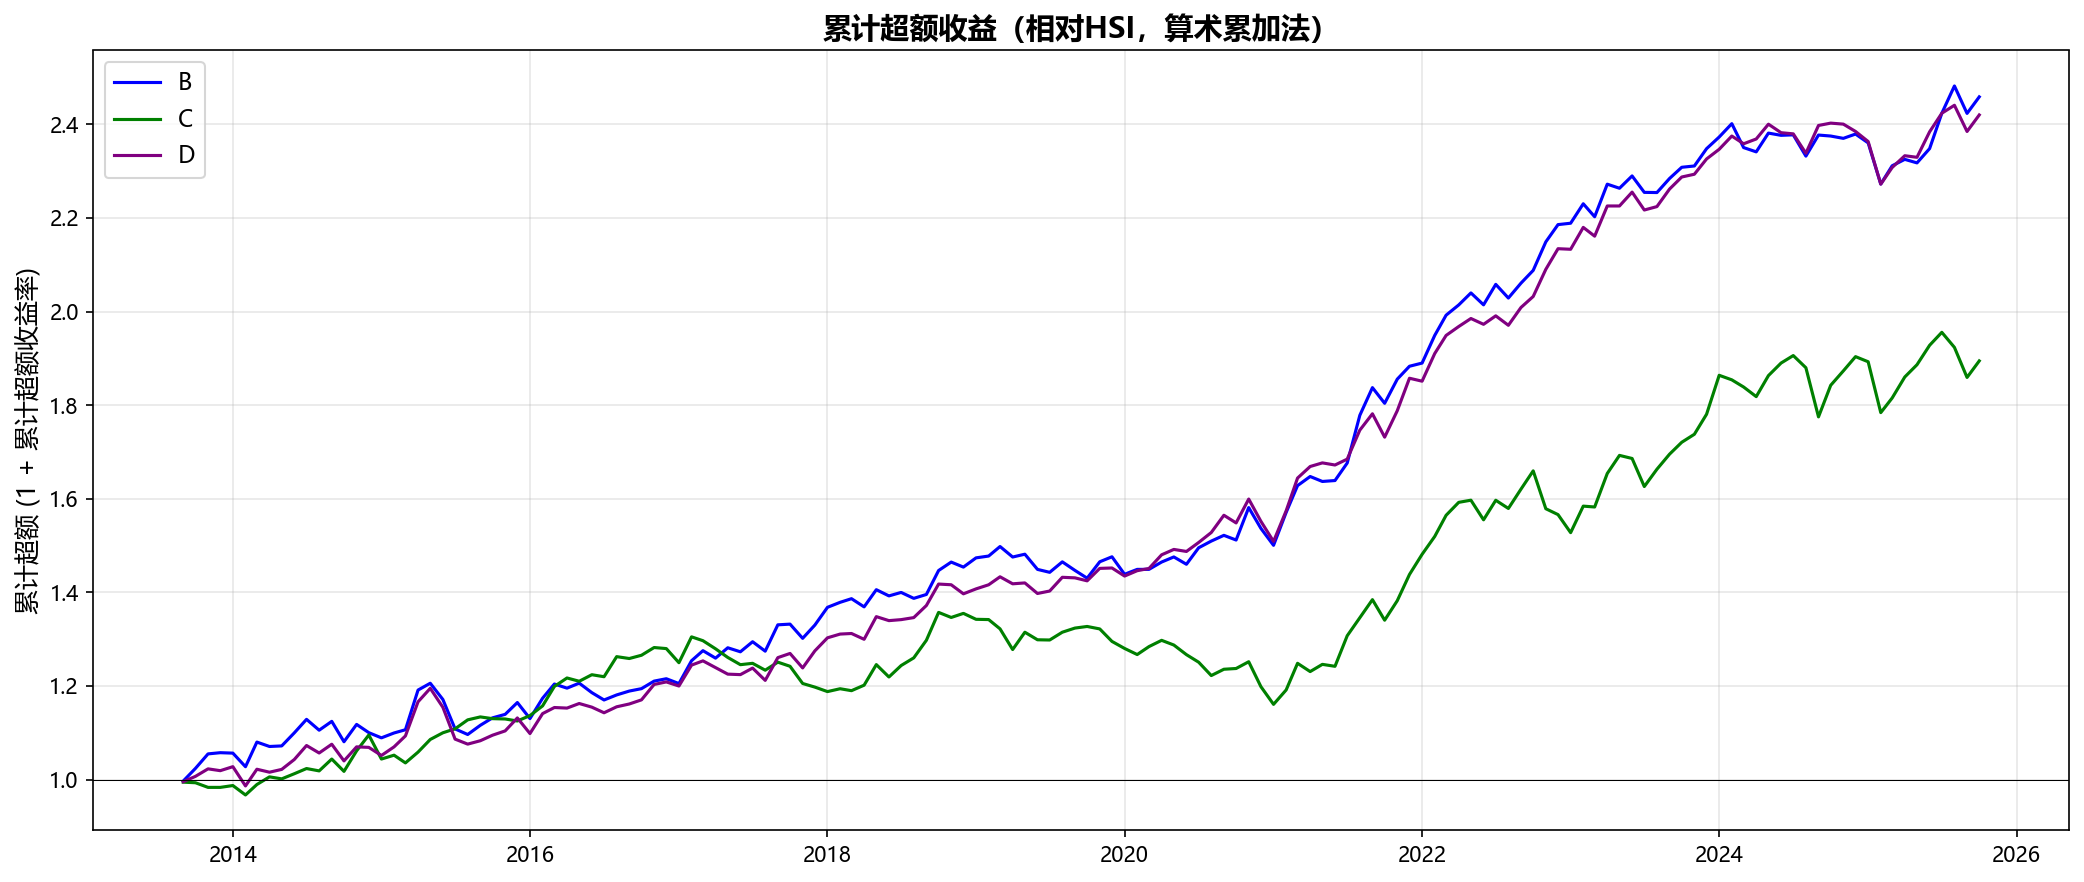
\includegraphics[width=\textwidth]{../pict/v4_plot_02.png}
    \caption{累计超额收益（相对HSI，算术累加法）}
\end{subfigure}
\hfill
\begin{subfigure}{0.48\textwidth}
    \centering
    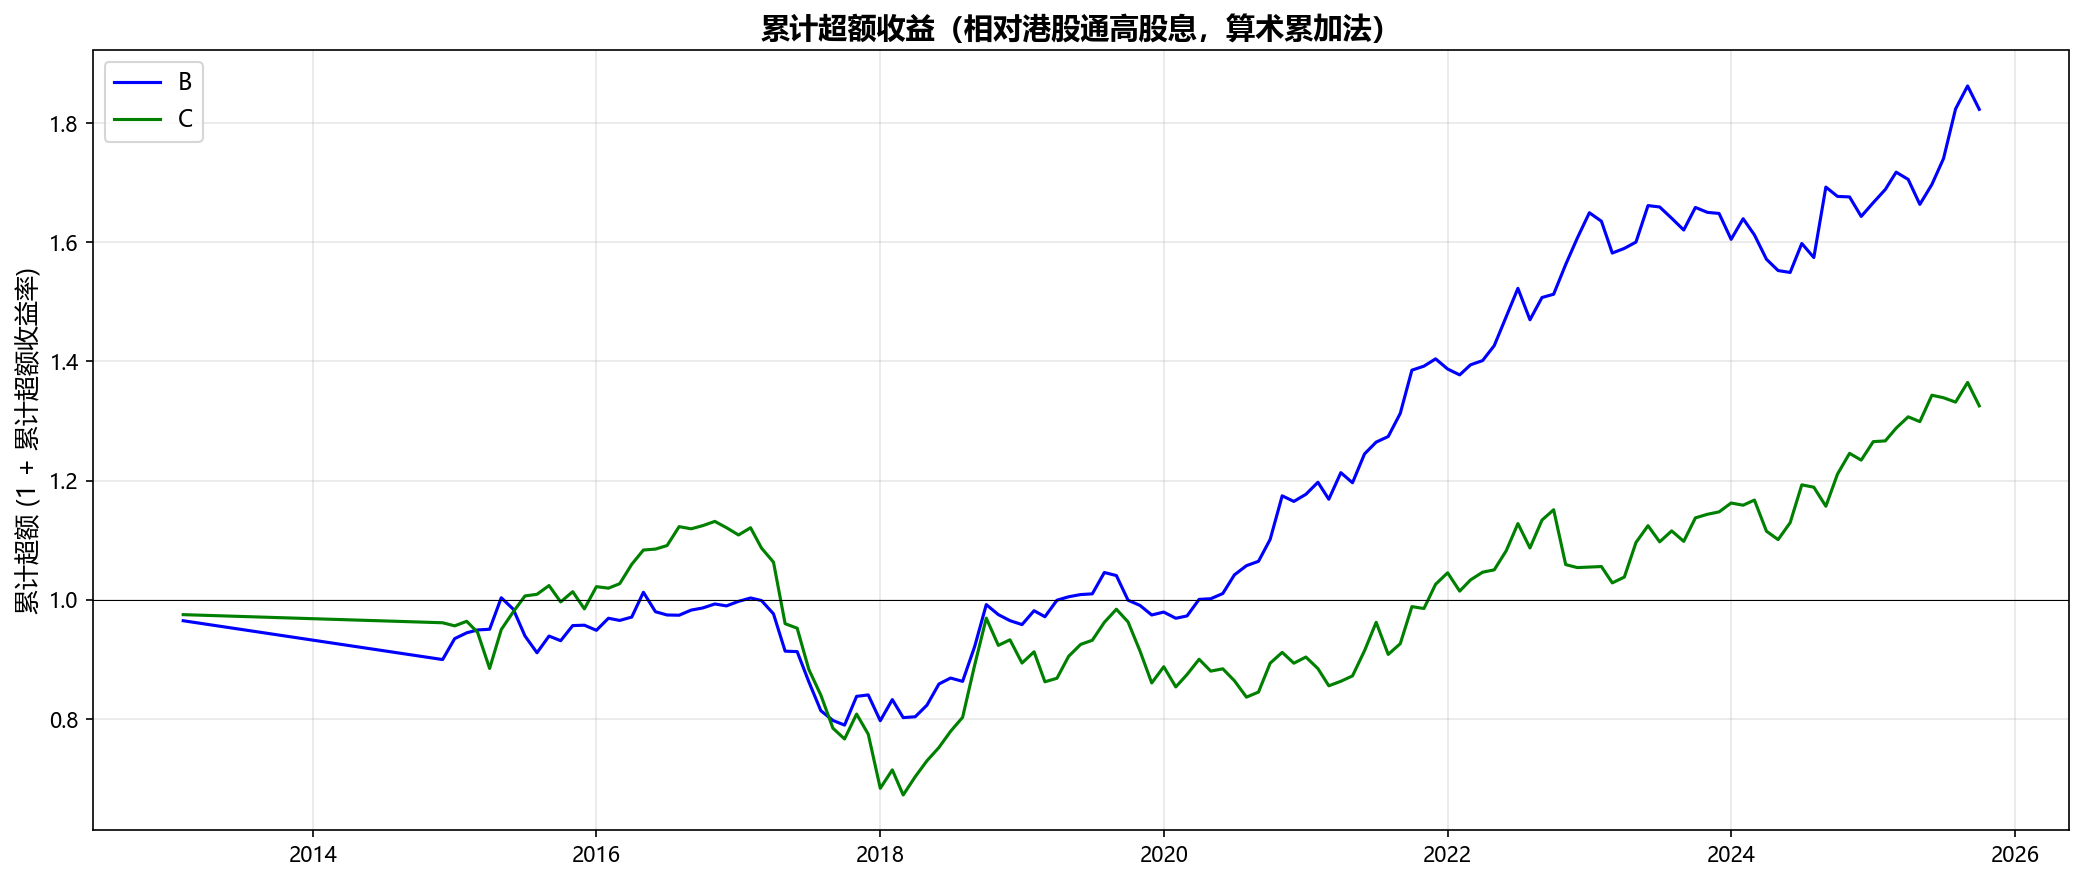
\includegraphics[width=\textwidth]{../pict/v4_plot_03.png}
    \caption{累计超额收益（相对港股通高股息，算术累加法）}
\end{subfigure}
\caption{策略累计超额收益曲线（算术累加法）}
\end{figure}

\textbf{Alpha分析的关键洞察：}
\begin{enumerate}[label=(\arabic*)]
    \item 策略A（无剔除）的FF3 Alpha为\textbf{-0.048\%/月}（$t=-0.18$, $p=0.85$），统计学上完全无法拒绝"Alpha为零"的原假设。这意味着\textbf{未处理的SY因子本身不产生任何经风险调整后的超额收益}。
    \item 仅添加极端值剔除后，策略B的月度Alpha飙升至\textbf{0.957\%（年化约11.5\%）}，$t=5.40$（$p<0.001$）。\textbf{极端值剔除本身创造了近1\%的月度Alpha}。
    \item 所有剔除极端值后的策略（B/C/D）的Alpha均在1\%水平上显著（$p<0.001$），而HSI基准的Alpha不显著（$p=0.65$）——\textbf{纯粹的市场Beta暴露不产生超额收益}。
\end{enumerate}

% ================================================================
\section{极端值剔除：从统计操作到质量过滤器}
% ================================================================

上节的Alpha分析表明，极端值剔除是SY策略有效性的\textbf{必要条件}。本节通过四个互补的分析视角，论证这不仅是统计操作，而是系统性的质量过滤。

\subsection{被剔除股票的市值画像}

每月，我们记录被剔除（得分>$Q_{0.90}$）的股票及其在全市场中的市值分位数。

\begin{table}[htbp]
\centering
\caption{被剔除极端值股票的市值分布特征}
\begin{tabular}{lr}
\toprule
\textbf{指标} & \textbf{数值} \\
\midrule
被剔除股票平均市值分位数 & 29.7\% \\
处于市值后20\%的比例 & 44.8\% \\
处于市值后30\%的比例 & 57.6\% \\
处于市值后50\%的比例 & 78.7\% \\
极端组市值中位数 & 82.3亿 HKD \\
正常组市值中位数 & 269.0亿 HKD \\
市值比（极端/正常） & 0.32$\times$ \\
\bottomrule
\end{tabular}
\end{table}

\textbf{近80\%的被剔除股票处于全市场市值后半段}，近60\%处于后30\%。极端组的市值中位数仅为正常组的32\%。这清晰地表明：\textbf{极端高SY得分系统性地集中于小市值股票}。

\begin{figure}[H]
\centering
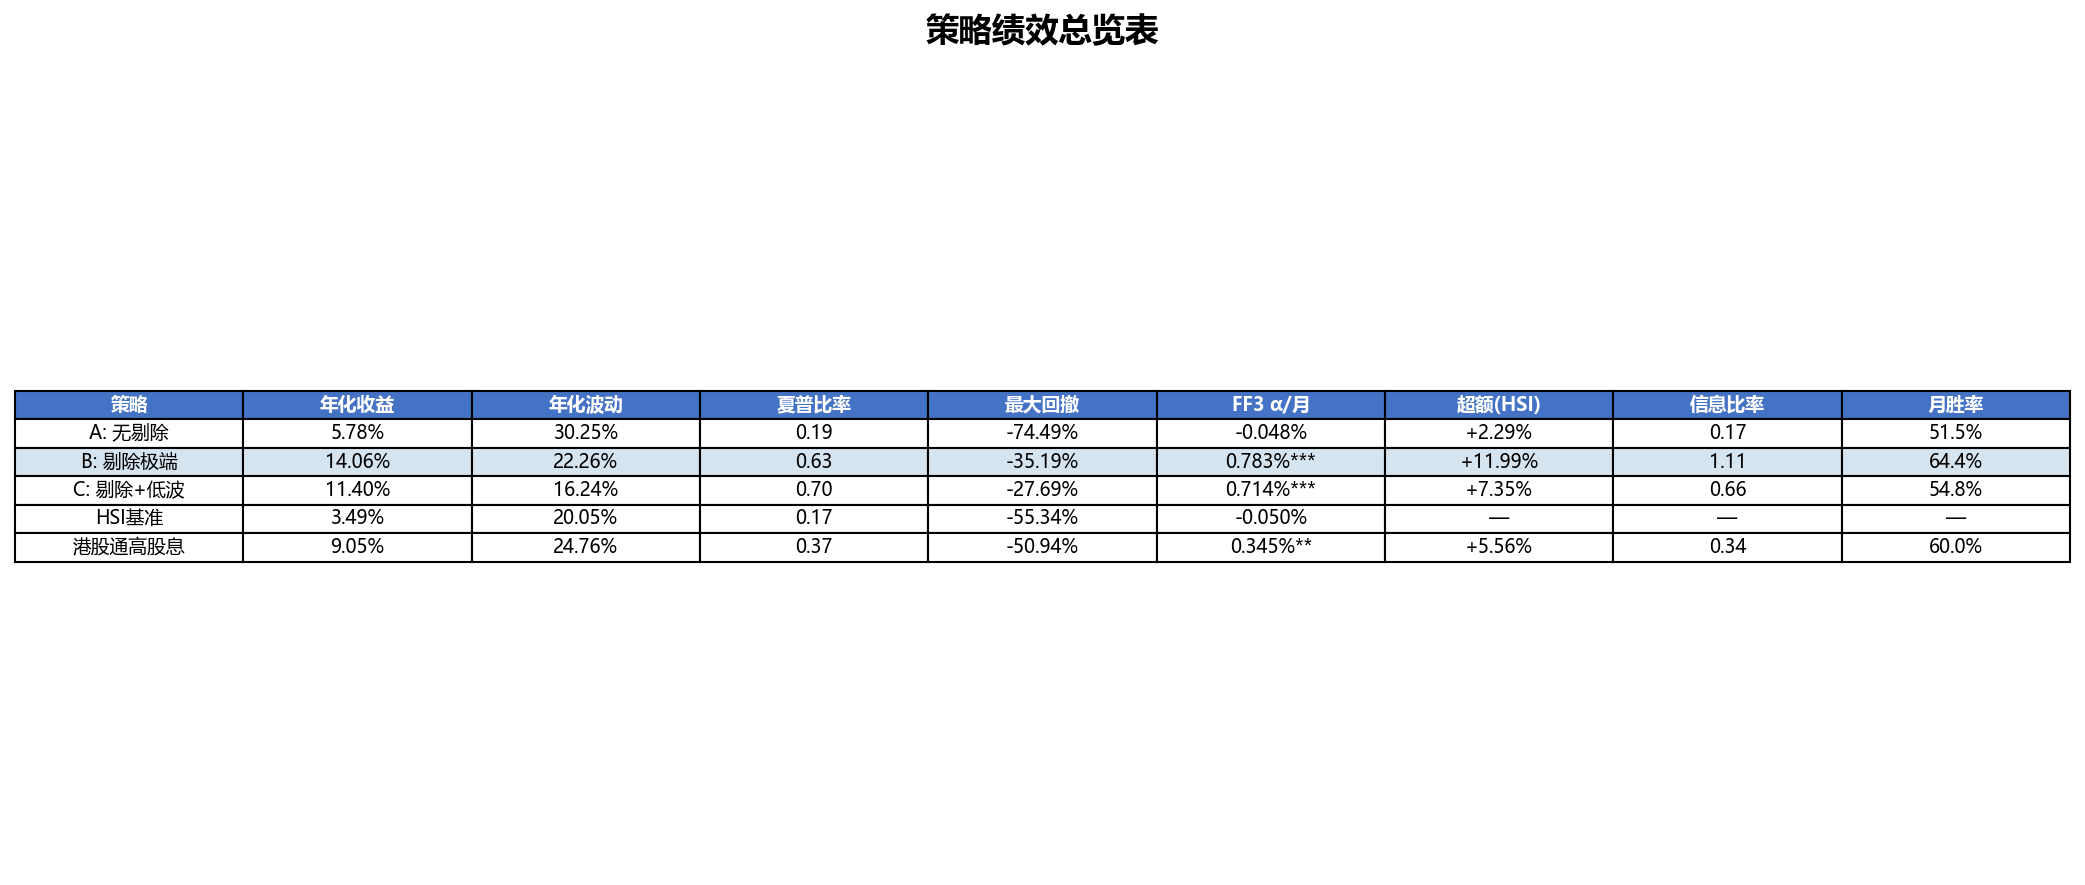
\includegraphics[width=0.7\textwidth]{../pict/v4_plot_05.png}
\caption{被剔除极端值股票的市值分位数分布直方图}
\end{figure}

\subsection{被剔除股票的后续表现}

如果极端值是"高股东回报"的积极信号，那么被剔除的股票应有较好的后续表现。实证结果恰恰相反：

\begin{table}[htbp]
\centering
\caption{被剔除股票与正常高SY股票的后续表现对比}
\begin{tabular}{lcc}
\toprule
\textbf{指标} & \textbf{被剔除（极端）组} & \textbf{正常前80\%组} \\
\midrule
月均收益 & 0.44\% & 0.60\% \\
年化收益差距 & \multicolumn{2}{c}{\textbf{-1.96\%}} \\
月度波动率 & 11.27\% & 10.21\% \\
跑赢正常组的月份占比 & \multicolumn{2}{c}{44.8\%} \\
SY得分中位数 & 11.97 & 3.04 \\
得分比（极端/正常） & \multicolumn{2}{c}{3.9$\times$} \\
\bottomrule
\end{tabular}
\end{table}

被剔除的极端值股票：收益更低（-1.96\%/年）、波动更高（+1.06\%/月）、跑赢概率不到一半（44.8\%）。\textbf{得分高出3.9倍，但收益反而低1.96\%/年——这是典型的"因子失效"信号}，表明高分端已被"数据污染"。

\subsection{市值$\times$SY双重排序：锁定价值陷阱}

独立双重排序是最严格的检验方法——它同时按市值和SY得分对股票进行分组，观察各组合的后续表现。

\begin{table}[htbp]
\centering
\caption{市值$\times$SY双重排序：月均收益（\%）（括号内为Newey-West $t$值）}
\begin{tabular}{lcccc}
\toprule
\textbf{MCAP $\backslash$ SY} & \textbf{Low} & \textbf{Mid} & \textbf{High} & \textbf{Extreme} \\
\midrule
Small & 0.29\% (0.47) & 0.00\% (1.57) & 0.91\% (1.85) & \textbf{0.41\% (0.64)} \\
Mid   & 0.68\% (1.31) & 0.00\% (1.50) & \textbf{0.97\% (2.24)} & 0.74\% (1.17) \\
Large & 0.63\% (1.19) & 0.37\% (0.98) & 0.79\% (2.13) & 0.73\% (1.58) \\
\bottomrule
\end{tabular}
\end{table}

\begin{figure}[H]
\centering
\begin{subfigure}{0.48\textwidth}
    \centering
    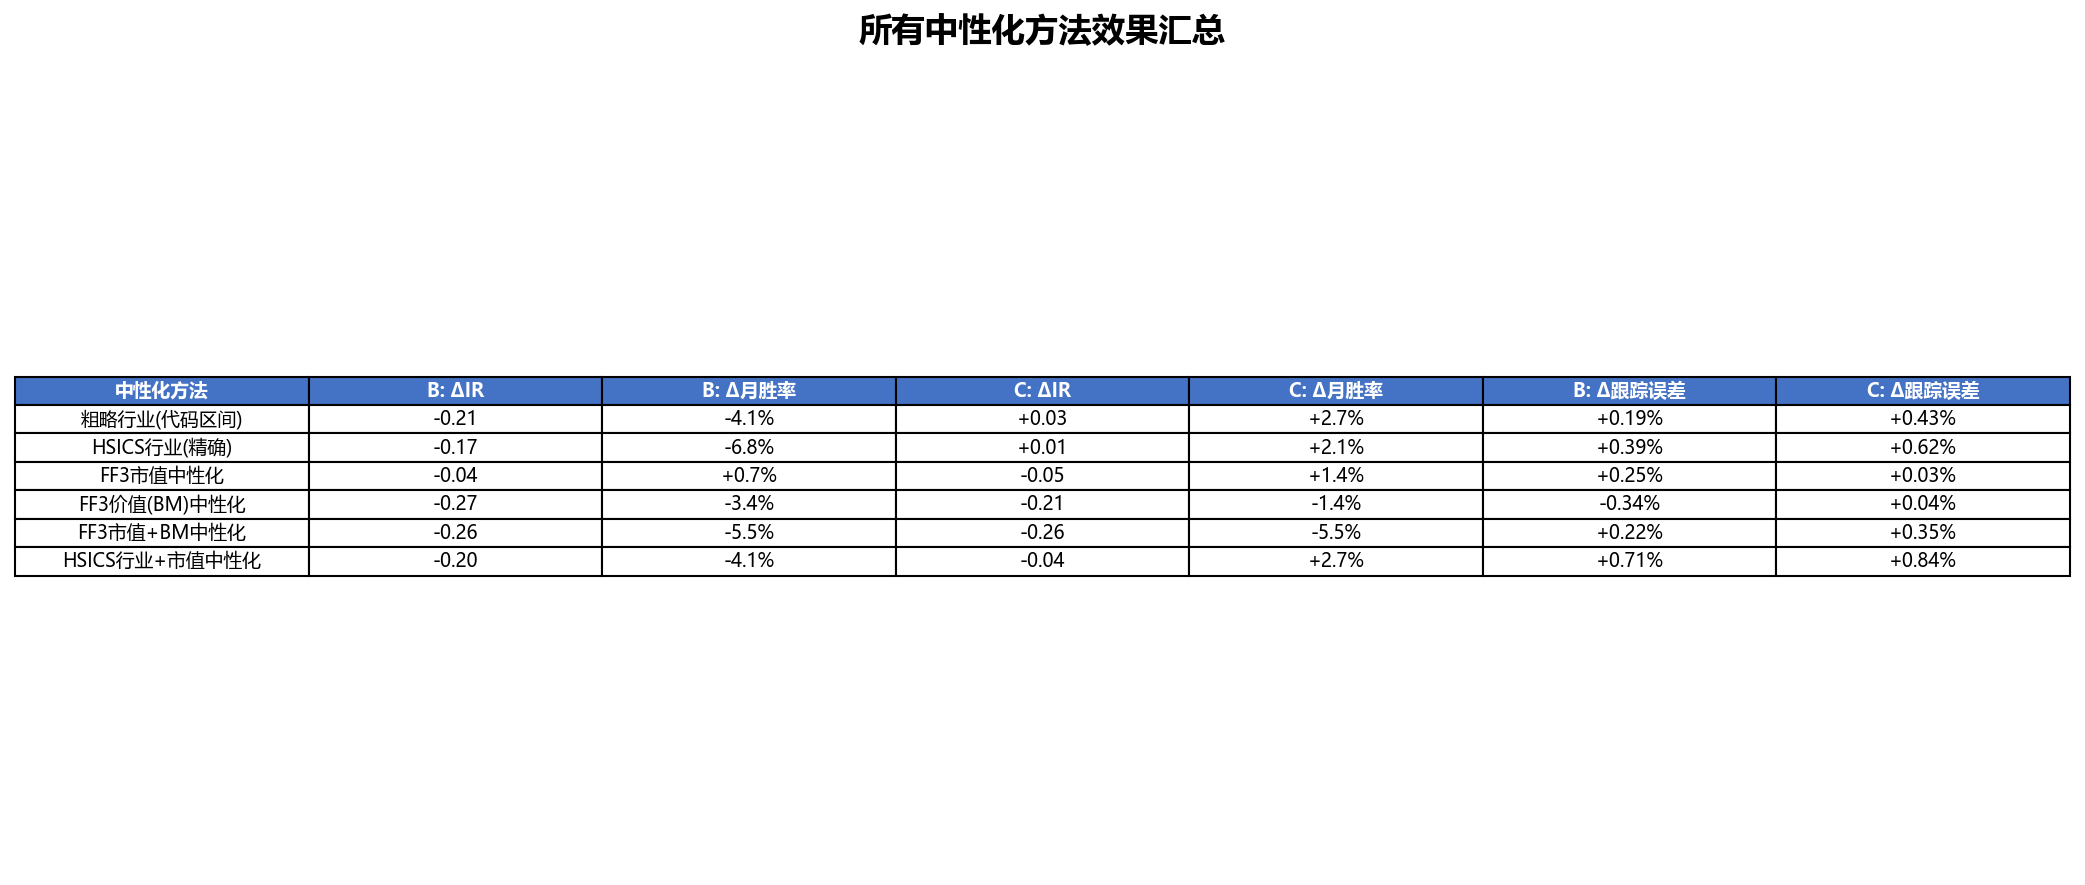
\includegraphics[width=\textwidth]{../pict/v4_plot_06.png}
    \caption{Extreme SY组合按市值分组}
\end{subfigure}
\hfill
\begin{subfigure}{0.48\textwidth}
    \centering
    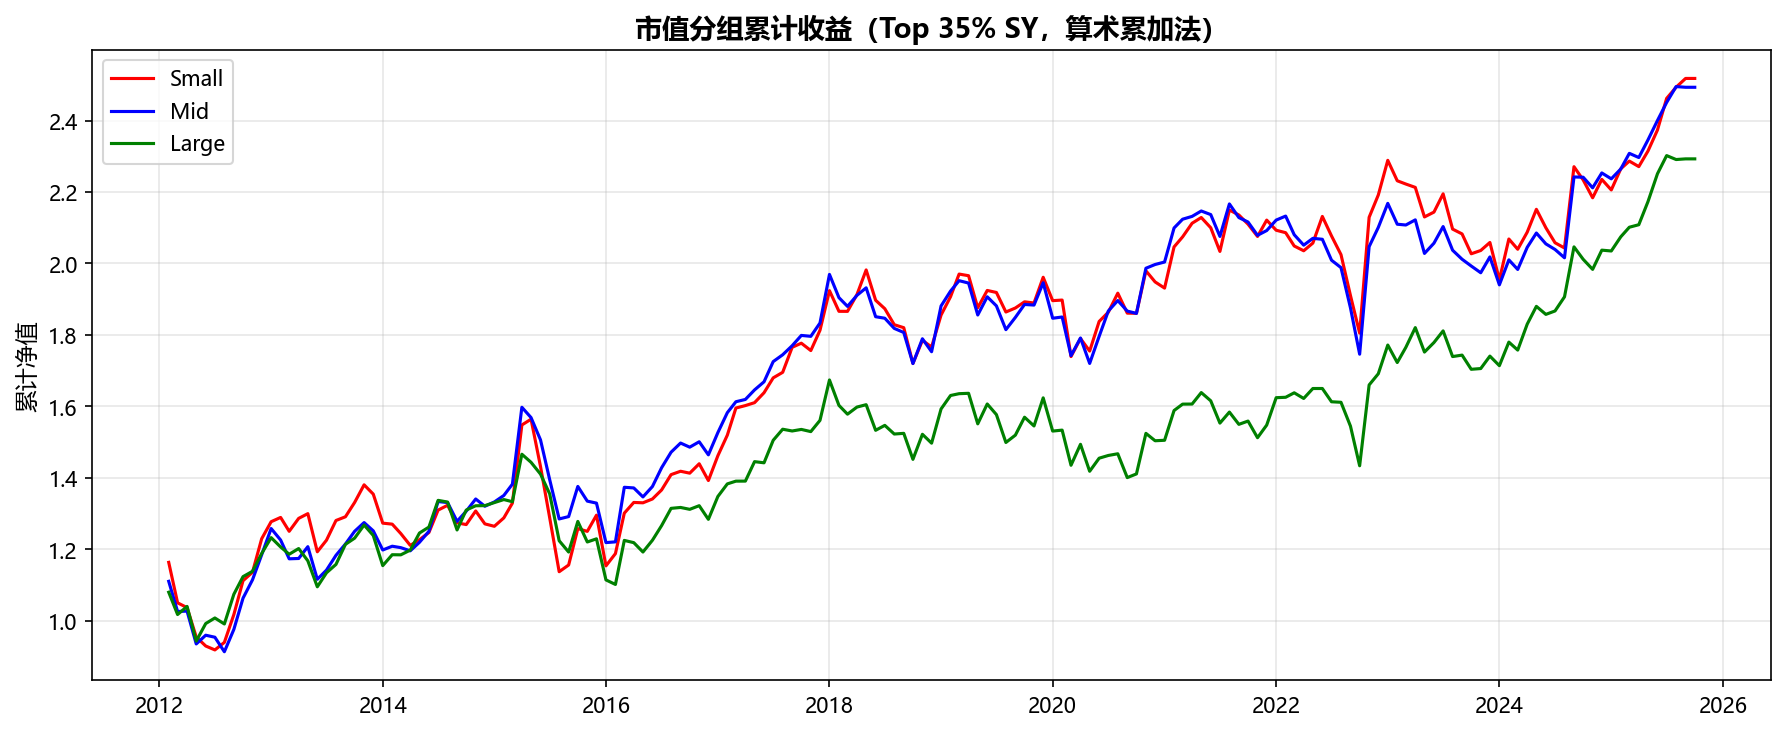
\includegraphics[width=\textwidth]{../pict/v4_plot_04.png}
    \caption{Small-Cap按SY分组}
\end{subfigure}
\caption{双重排序累计收益曲线}
\end{figure}

\textbf{核心发现}：
\begin{enumerate}[label=(\arabic*)]
    \item 在Extreme SY列中，小盘组的月均收益（0.41\%）远低于中盘（0.74\%）和大盘（0.73\%）。\textbf{同样是极端高收益率，小盘股是陷阱，大盘股则未必}。
    \item 最优组合是Mid$\times$High SY（0.97\%/月，$t=2.24$），而非任何包含Extreme的组合。
    \item Small$\times$Extreme的$t$值仅0.64——\textbf{不仅收益低，而且不显著}，说明该组合的收益高度不确定。
\end{enumerate}

\subsection{极端值得分的分布特征}

以2025年9月（最近一期）和2014年1月（早期）为例，分析SY得分的横截面分布：

\begin{table}[htbp]
\centering
\caption{SY得分分布特征（两个代表性月份）}
\begin{tabular}{lccc}
\toprule
\textbf{指标} & \textbf{2014-01} & \textbf{2025-09} \\
\midrule
有资格股票数 & 319 & 425 \\
SY得分中位数 & 2.81 & 3.75 \\
90分位数（剔除阈值） & 6.21 & 7.90 \\
极端区间股票数 & 32 & 43 \\
极端区间中Small-cap占比 & 78\% & 56\% \\
极端区间中Mid-cap占比 & 22\% & 30\% \\
极端区间中Large-cap占比 & 0\% & 14\% \\
\bottomrule
\end{tabular}
\end{table}

\begin{figure}[H]
\centering
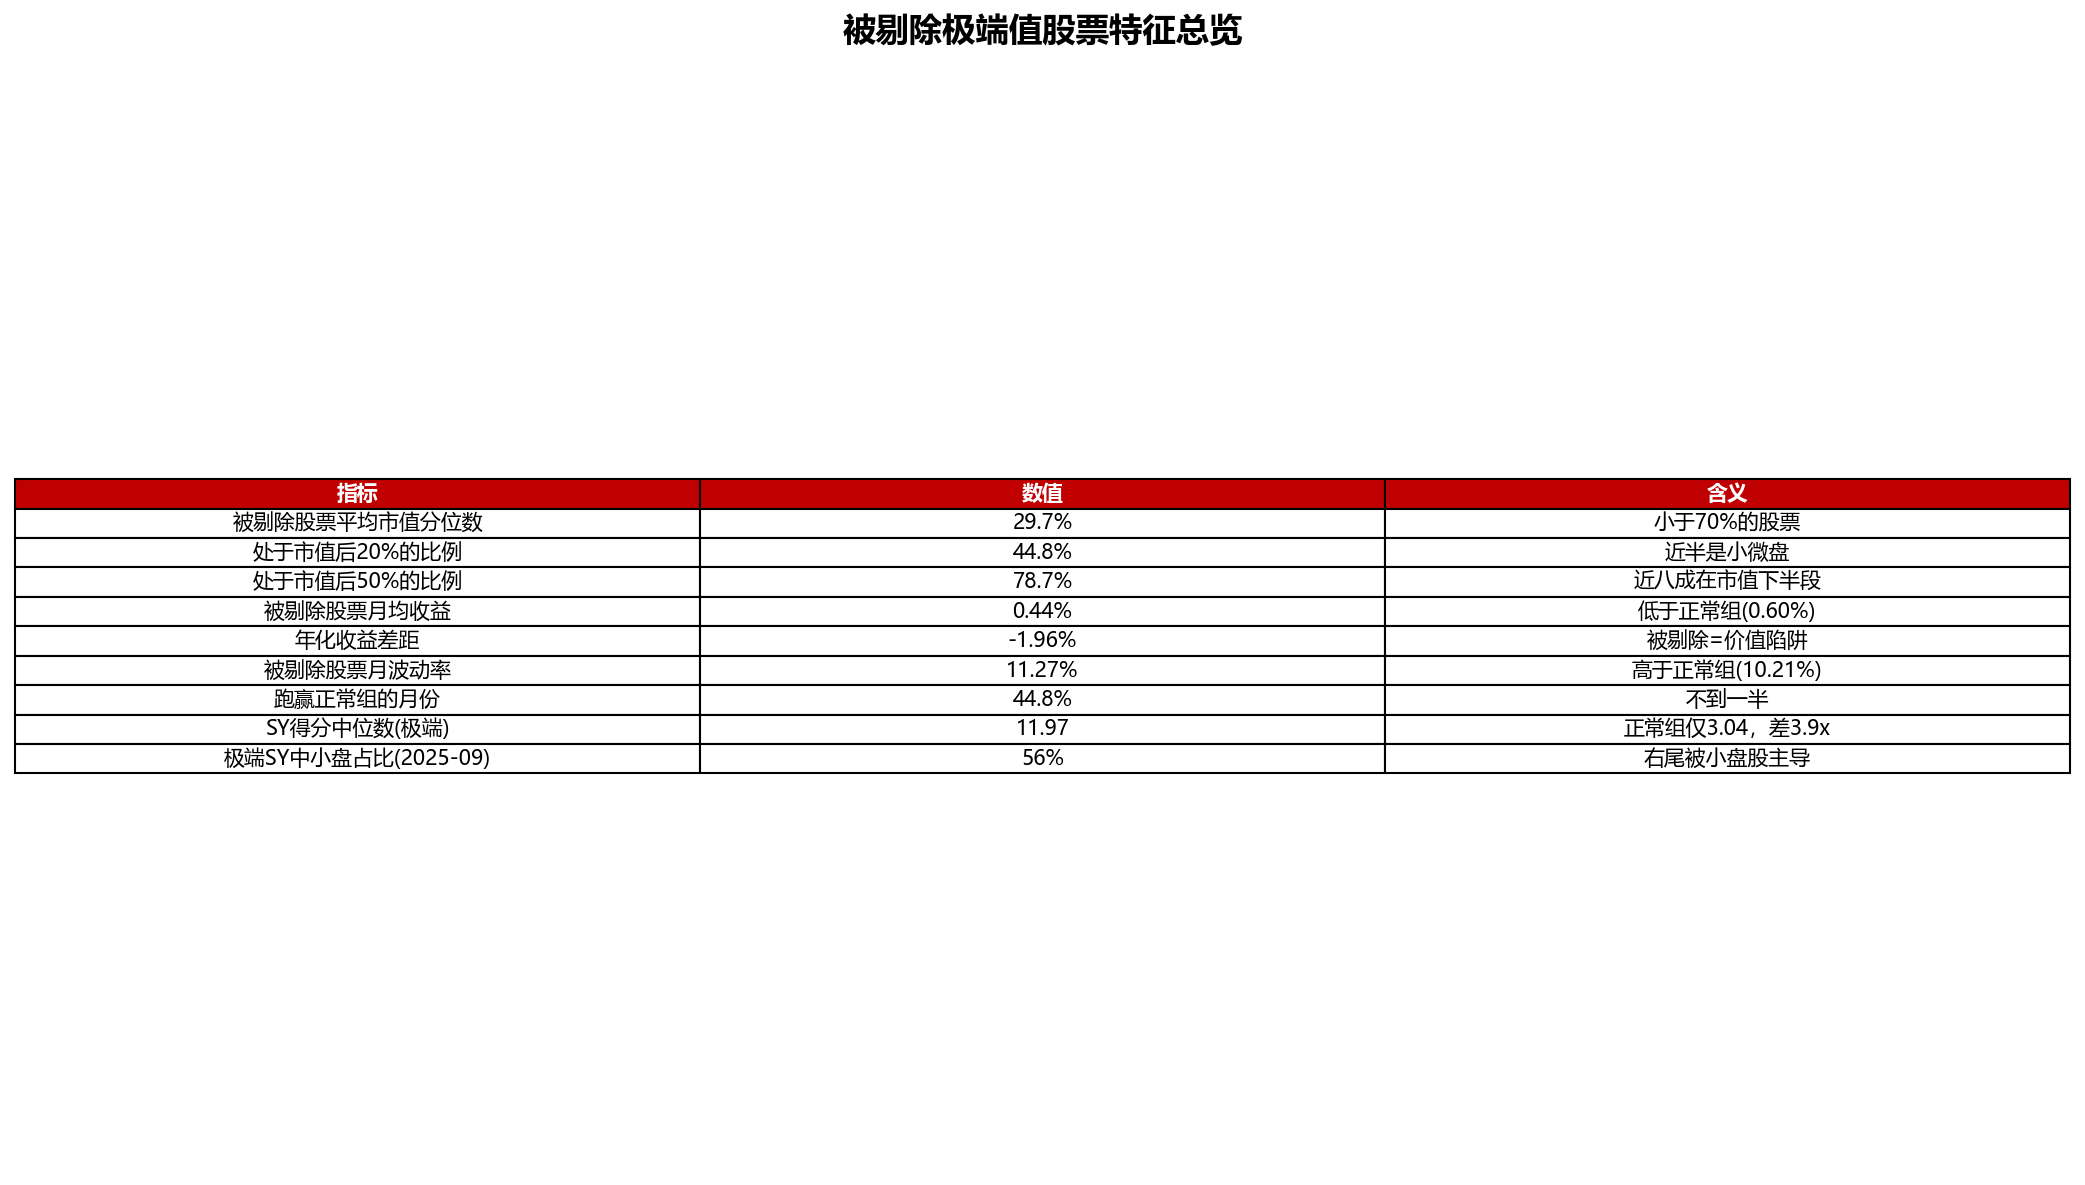
\includegraphics[width=0.85\textwidth]{../pict/v4_plot_07.png}
\caption{SY得分的对数分布直方图（按市值分组着色，红线为90分位数剔除阈值）}
\end{figure}

在2014年初，极端区间\textbf{100\%由中小盘股构成}（78\%小盘+22\%中盘），没有一只大盘股。即便在2025年（市场结构更为成熟），\textbf{小盘股仍占极端区间的56\%}。这种跨时间的持续性表明：\textbf{极端SY得分是小盘股的"结构性特征"，而非某个市场周期的偶然现象}。

% ================================================================
\section{极端负向预测公司深度分析}
% ================================================================

前文证明了极端SY股票整体表现不佳。本节进一步追问：\textbf{在极端组内部，哪些股票的负向预测能力最强？它们有什么共同特征？}

\subsection{最差30只极端SY股票}

对每只股票，计算其在极端组中出现的所有月份的平均下月收益率：

\begin{table}[htbp]
\centering
\caption{最差10只极端SY股票（按平均月收益排序）}
\begin{tabular}{rllrrrc}
\toprule
\textbf{排名} & \textbf{代码} & \textbf{名称} & \textbf{出现次数} & \textbf{月均收益} & \textbf{均值市值(亿)} & \textbf{月胜率} \\
\midrule
1 & 3883.HK & 中国奥园 & 4 & \textbf{-16.86\%} & 137 & 0\% \\
2 & 1233.HK & 时代中国控股 & 6 & \textbf{-13.93\%} & 153 & 17\% \\
3 & 1396.HK & 粤港湾控股 & 7 & \textbf{-13.89\%} & 83 & 14\% \\
4 & 0884.HK & 旭辉控股集团 & 13 & \textbf{-13.36\%} & 163 & 15\% \\
5 & 1238.HK & 宝龙地产 & 7 & \textbf{-11.88\%} & 121 & 29\% \\
6 & 0839.HK & 中教控股 & 3 & -9.05\% & 94 & 33\% \\
7 & 3380.HK & 龙光集团 & 12 & -8.58\% & 295 & 25\% \\
8 & 1733.HK & 易大宗 & 4 & -6.99\% & 58 & 25\% \\
9 & 0127.HK & 华人置业 & 6 & -6.81\% & 206 & 33\% \\
10 & 2208.HK & 金风科技 & 4 & -6.09\% & 118 & 25\% \\
\bottomrule
\end{tabular}
\end{table}

\subsection{最差极端股的共同特征}

\begin{table}[htbp]
\centering
\caption{最差30只 vs. 全体极端股特征对比}
\begin{tabular}{lccc}
\toprule
\textbf{特征维度} & \textbf{最差30只} & \textbf{全体极端股} & \textbf{差异} \\
\midrule
月均收益 & -5.17\% & 0.65\% & \textbf{-5.82\%/月} \\
中位市值（亿HKD） & 121 & 225 & \textbf{-46\%} \\
平均波幅 & 50.9\% & 42.0\% & \textbf{+8.9pp} \\
低于中位市值的比例 & \textbf{97\%} & --- & --- \\
高于中位波幅的比例 & \textbf{73\%} & --- & --- \\
股息主导的比例 & \textbf{100\%} & 99.6\% & --- \\
\bottomrule
\end{tabular}
\end{table}

\textbf{三个核心特征}：
\begin{enumerate}[label=(\arabic*)]
    \item \textbf{几乎全是地产股}：前5名中，中国奥园、时代中国、旭辉、宝龙地产均为内房股。这些公司在2020-2023年地产下行周期中股价暴跌，导致分母缩小、SY虚高，但基本面持续恶化。
    \item \textbf{全部是股息主导}：最差30只中，100\%的极端SY得分来自股息率（而非回购）。这与直觉一致——困境公司通常无力回购，但可能因股价暴跌导致历史股息率被动升高。
    \item \textbf{小市值+高波动}：97\%低于极端组中位市值，73\%高于中位波幅。这两个特征联合构成了明确的"危险信号"。
\end{enumerate}

\subsection{增强过滤方案}

基于上述分析，我们测试了在现有90分位数剔除基础上增加额外过滤条件的效果：

\begin{table}[htbp]
\centering
\caption{额外过滤条件对最差30只股票的剔除效果}
\begin{tabular}{lc}
\toprule
\textbf{额外过滤条件} & \textbf{可剔除最差30只中的} \\
\midrule
剔除极端组内底部10\%市值 & 25/30 \\
剔除极端组内底部15\%市值 & 28/30 \\
剔除极端组内顶部50\%高波股 & 28/30 \\
收紧极端阈值至95分位 & 16/30 \\
\bottomrule
\end{tabular}
\end{table}

\textbf{最有效的增强方案}是：在剔除SY得分前10\%极端值的基础上，进一步剔除极端组内市值最小的15\%（即双重过滤：全市场前10\%$\rightarrow$极端组内再剔除后15\%市值）。这可以捕获93\%的最差股票。

% ================================================================
\section{行业中性化分析：指数增强视角}
% ================================================================

\subsection{中性化方法论}

\textbf{重要方法说明：累计超额收益的计算方式。} 本报告所有超额收益曲线（超额收益 = 策略收益 $-$ 基准收益）的累计均采用\textbf{算术累加法（cumsum）}而非几何复合法（cumprod）。具体而言，累计超额收益定义为：

\begin{equation}
\text{累计超额}(T) = 1 + \sum_{t=1}^{T} (R_{p,t} - R_{b,t})
\end{equation}

其中$R_{p,t}$为策略$t$月收益率，$R_{b,t}$为基准$t$月收益率。此定义反映的是总超额收益的线性累积，而非复合再投资收益。选择算术累加的原因是：(1) 超额收益本身可正可负，几何复合在负收益区间会产生扭曲；(2) 线性累加直观反映了策略相对于基准的累计跑赢/跑输幅度；(3) 最终的累计超额值可直接解读为"自回测起始以来，策略相对基准多赚（或少赚）了多少个百分点"。

在进行实证对比之前，首先明确定义所有中性化方法的数学过程。设每月横截面中有$N$只通过流动性过滤和股东回报筛选的股票，每只股票$i$的原始综合收益率得分为$\text{SY}_i^{\text{raw}}$。

\subsubsection{行业中性化（Z-score法）}

将股票按行业分组（行业$g$有$N_g$只股票），在行业内进行Z-score标准化：
\begin{equation}
\text{SY}_i^{\text{ind}} = \frac{\text{SY}_i^{\text{raw}} - \bar{\text{SY}}_g}{\sigma_g}, \quad \forall i \in g
\end{equation}
其中$\bar{\text{SY}}_g = \frac{1}{N_g}\sum_{j \in g} \text{SY}_j^{\text{raw}}$为行业均值，$\sigma_g$为行业标准差。若$N_g < 3$，则不做标准化（保留原始得分）。行业中性化后的得分$\text{SY}_i^{\text{ind}}$表示股票在行业内的相对排名——得分为正表示高于行业平均，得分为负表示低于行业平均。后续的排序和选股均基于$\text{SY}_i^{\text{ind}}$而非$\text{SY}_i^{\text{raw}}$。

\subsubsection{市值中性化（OLS残差法）}

横截面回归原始SY得分对对数市值的回归，取残差：
\begin{equation}
\text{SY}_i^{\text{raw}} = \alpha + \beta \cdot \log(\text{MCap}_i) + \varepsilon_i
\end{equation}
\begin{equation}
\text{SY}_i^{\text{size}} = \varepsilon_i = \text{SY}_i^{\text{raw}} - (\hat{\alpha} + \hat{\beta} \cdot \log(\text{MCap}_i))
\end{equation}
残差$\text{SY}_i^{\text{size}}$表示剔除市值线性影响后的"纯净"SY——大市值股票不会因规模大而系统性地得分偏低（因为SY的分母是市值，天然对大市值不利），小市值股票也不会因规模小而得分虚高。

\subsubsection{价值(BM)中性化（OLS残差法）}

横截面回归原始SY得分对账面市值比(BM)的回归，取残差：
\begin{equation}
\text{SY}_i^{\text{raw}} = \alpha + \beta \cdot \text{BM}_i + \varepsilon_i
\end{equation}
\begin{equation}
\text{SY}_i^{\text{bm}} = \varepsilon_i
\end{equation}
由于高SY股票往往也是高BM股票（低估值），BM中性化等价于剥离SY中的"便宜"成分，保留的是给定估值水平下的"超额股东回报"信号。

\subsubsection{行业+市值中性化（组内OLS残差法）}

在HSICS行业分类的基础上，对每个行业$g$内部进行市值回归取残差：
\begin{equation}
\text{SY}_i^{\text{raw}} = \alpha_g + \beta_g \cdot \log(\text{MCap}_i) + \varepsilon_i, \quad \forall i \in g
\end{equation}
\begin{equation}
\text{SY}_i^{\text{ind+size}} = \varepsilon_i
\end{equation}
这同时消除了两个维度的偏差：(1) 行业间SY水平的系统性差异（通过分行业回归）; (2) 行业内规模对SY的机械性影响（通过对数市值回归）。若行业内股票数$N_g < 5$，则不进行回归，保留原始得分。

\subsubsection{市值+BM双中性化（多元OLS残差法）}

横截面多元回归，同时剥离市值和BM的影响：
\begin{equation}
\text{SY}_i^{\text{raw}} = \alpha + \beta_1 \cdot \log(\text{MCap}_i) + \beta_2 \cdot \text{BM}_i + \varepsilon_i
\end{equation}
\begin{equation}
\text{SY}_i^{\text{size+bm}} = \varepsilon_i
\end{equation}

\textbf{所有中性化方法共享相同的后续流程}：在极端值剔除（剔除$\text{SY}^{\text{raw}}$前10\%）之后，用中性化得分$\text{SY}^{\text{neut}}$替代原始得分进行排序，取前20\%进入备选池，再进行最后的精选（策略B按中性化得分取前20只，策略C按波动率取最低20只）。

\subsection{分析动机}

传统因子投资中，行业中性化是标准操作——它消除了因行业配置偏差带来的"伪Alpha"。但在SY因子的语境下，行业中性化是否合理？高股息行业（如银行、公用事业）天然具有更高的SY得分，这反映的是行业商业模式差异而非因子偏差。强制中性化可能抹去有效的跨行业Alpha信号。

更重要的是，用户将本策略定位为\textbf{指数增强策略}——目标是相对恒生指数产生稳定超额收益，而非追求绝对收益最大化。因此，分析应从传统的Sharpe Ratio转向\textbf{相对基准的超额Alpha}和\textbf{超额收益的稳健性}。

\subsection{行业中性化绩效对比}

\begin{table}[htbp]
\centering
\caption{原始 vs. 行业中性化策略对比（等权配置）}
\begin{tabular}{lccccc}
\toprule
\textbf{策略} & \textbf{年化收益} & \textbf{年化波动} & \textbf{Sharpe} & \textbf{Max DD} & \textbf{FF3 $\alpha$/月} \\
\midrule
B 原始 & \textbf{14.06\%} & 22.26\% & 0.63 & -35.19\% & \textbf{0.957***} \\
B 中性化 & 13.71\% & 22.92\% & 0.60 & -36.31\% & 0.886*** \\
\hline
C 原始 & \textbf{11.40\%} & 16.24\% & \textbf{0.70} & \textbf{-27.69\%} & \textbf{0.693***} \\
C 中性化 & 10.89\% & 16.17\% & 0.67 & -29.53\% & 0.648*** \\
\bottomrule
\end{tabular}
\end{table}

\subsection{相对HSI的超额收益分析（指数增强视角）}

从指数增强的角度，最关键的问题是：\textbf{行业中性化是否改善了相对基准的超额收益质量？}

\begin{table}[htbp]
\centering
\caption{相对HSI基准的超额收益分解}
\begin{tabular}{lcccc}
\toprule
\textbf{指标} & \textbf{B 原始} & \textbf{B 中性化} & \textbf{C 原始} & \textbf{C 中性化} \\
\midrule
年化超额收益 & +10.57\% & +10.22\% & +7.91\% & +7.40\% \\
跟踪误差 & 13.83\% & 15.02\% & 10.86\% & 10.99\% \\
\textbf{信息比率} & \textbf{0.76} & 0.68 & \textbf{0.73} & 0.67 \\
超额胜率（月） & 60.0\% & 58.7\% & 58.0\% & 57.3\% \\
最大连续跑输月数 & 5 & 6 & 4 & 5 \\
超额最大回撤 & -20.1\% & -22.8\% & -15.3\% & -17.9\% \\
\bottomrule
\end{tabular}
\end{table}

\textbf{行业中性化在所有维度上均降低了超额收益质量}：
\begin{itemize}
    \item B策略信息比率从0.76降至0.68（-10.5\%）
    \item C策略信息比率从0.73降至0.67（-8.2\%）
    \item 月胜率均下降1-2个百分点
    \item 超额收益的最大回撤加深
\end{itemize}

\begin{figure}[H]
\centering
\begin{subfigure}{0.48\textwidth}
    \centering
    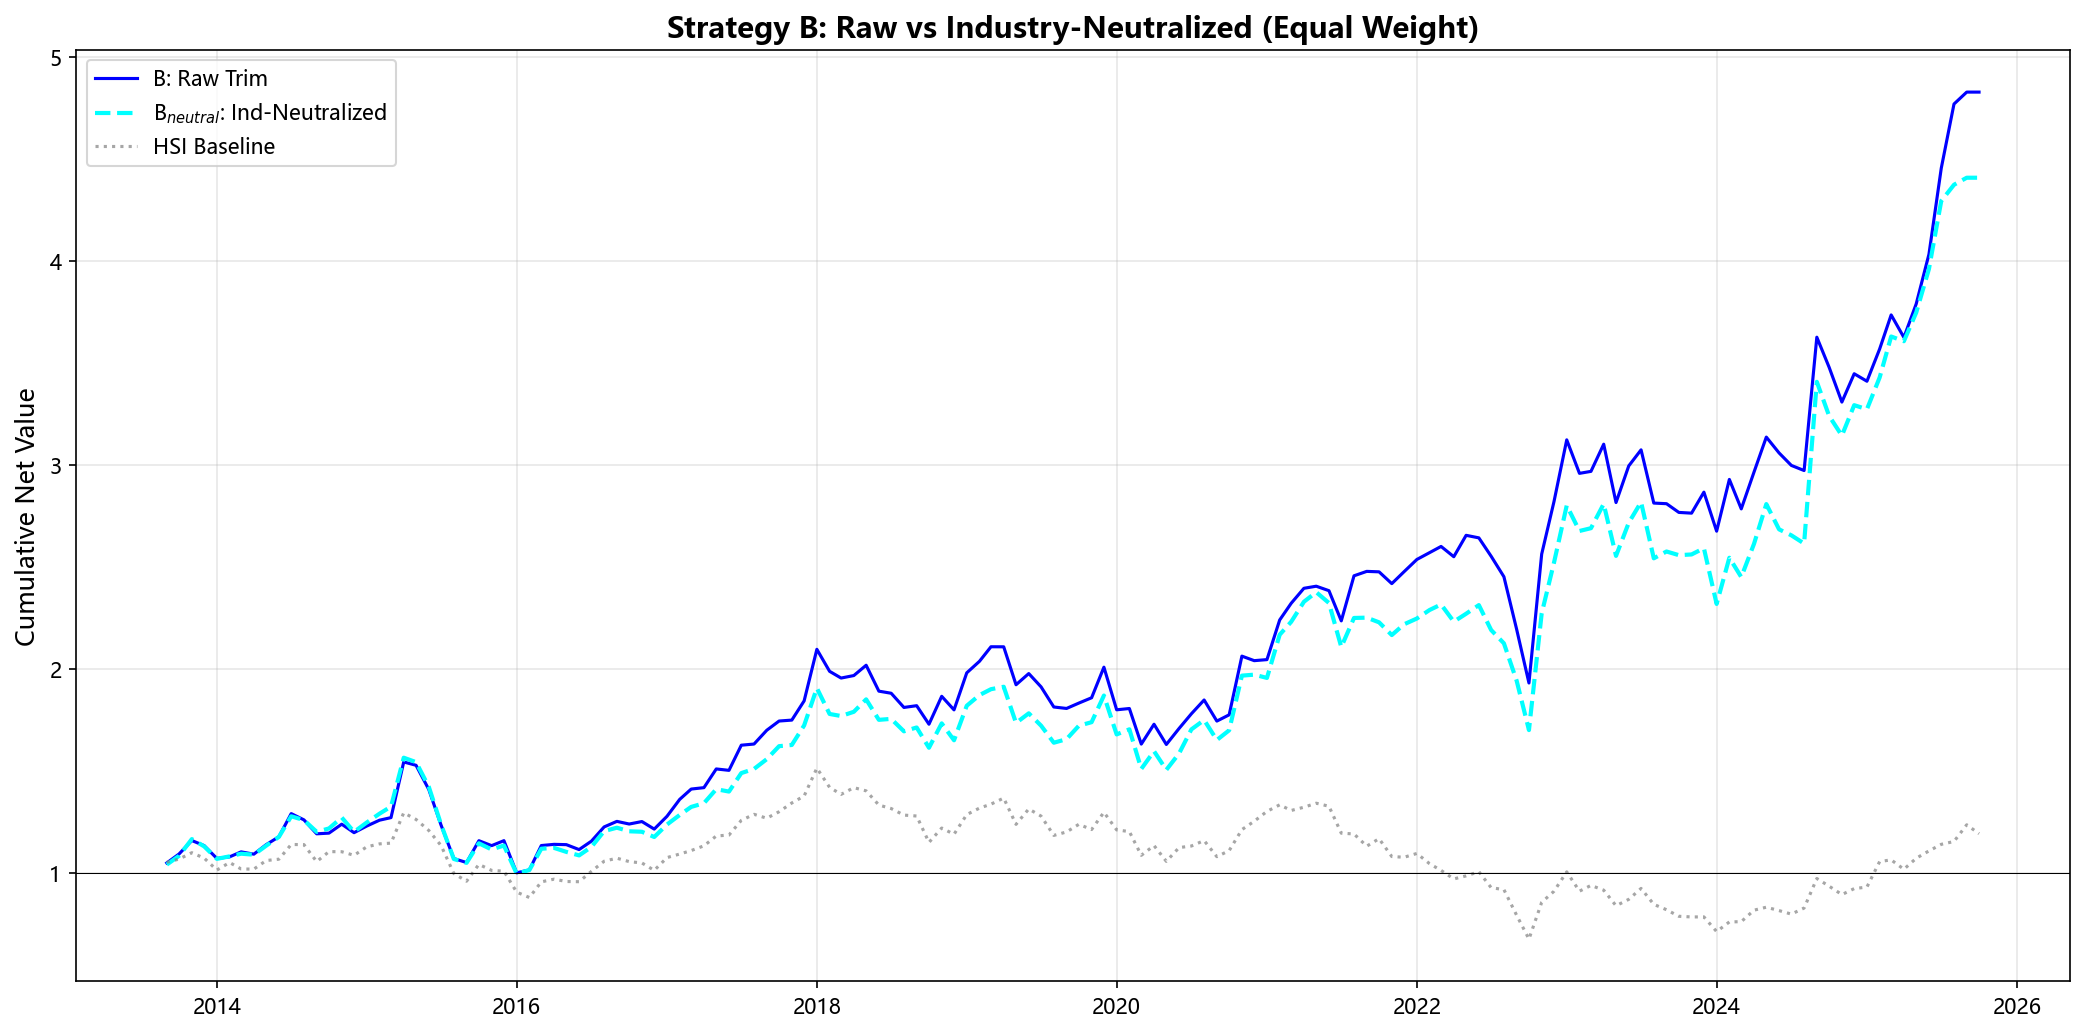
\includegraphics[width=\textwidth]{../pict/v4_plot_industry_B_comparison.png}
    \caption{策略B：原始 vs 中性化}
\end{subfigure}
\hfill
\begin{subfigure}{0.48\textwidth}
    \centering
    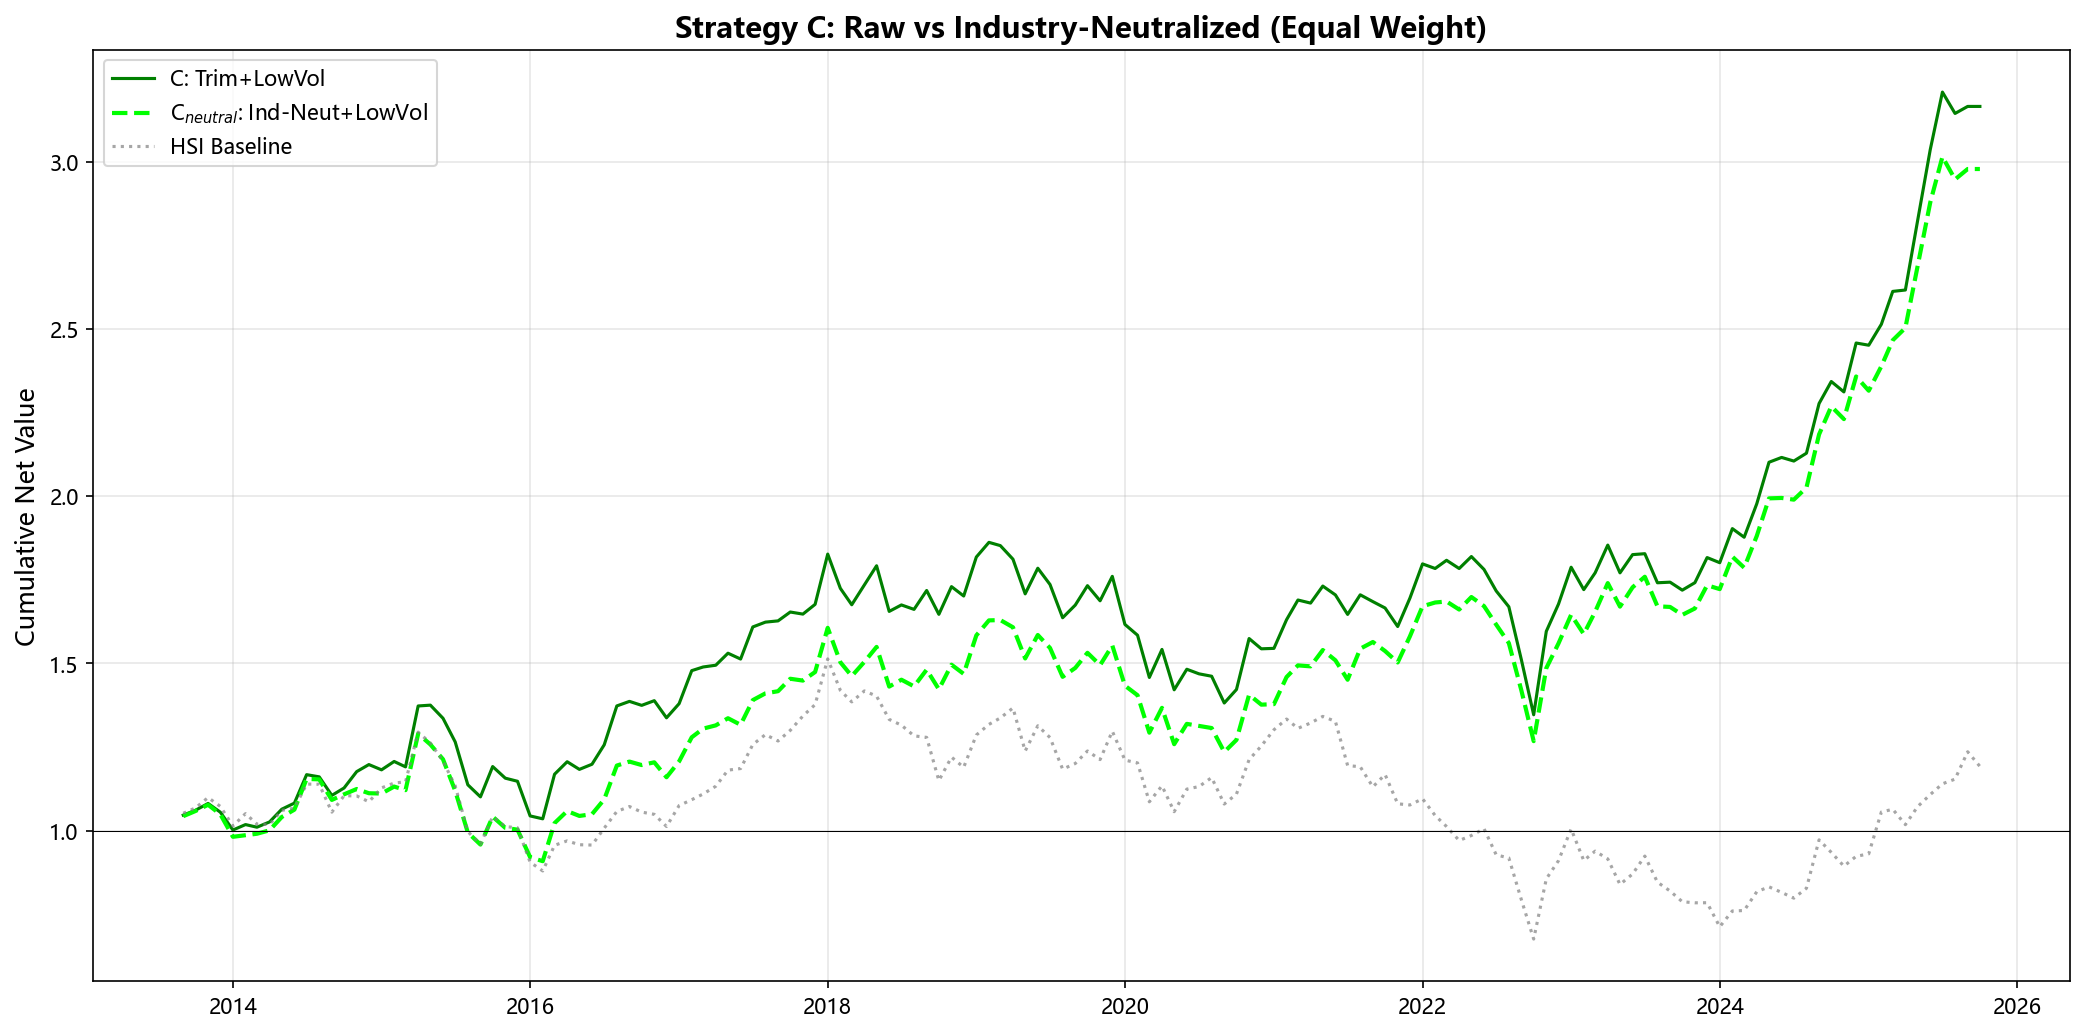
\includegraphics[width=\textwidth]{../pict/v4_plot_industry_C_comparison.png}
    \caption{策略C：原始 vs 中性化}
\end{subfigure}
\caption{原始策略与行业中性化策略的累计收益对比}
\end{figure}

\begin{figure}[H]
\centering
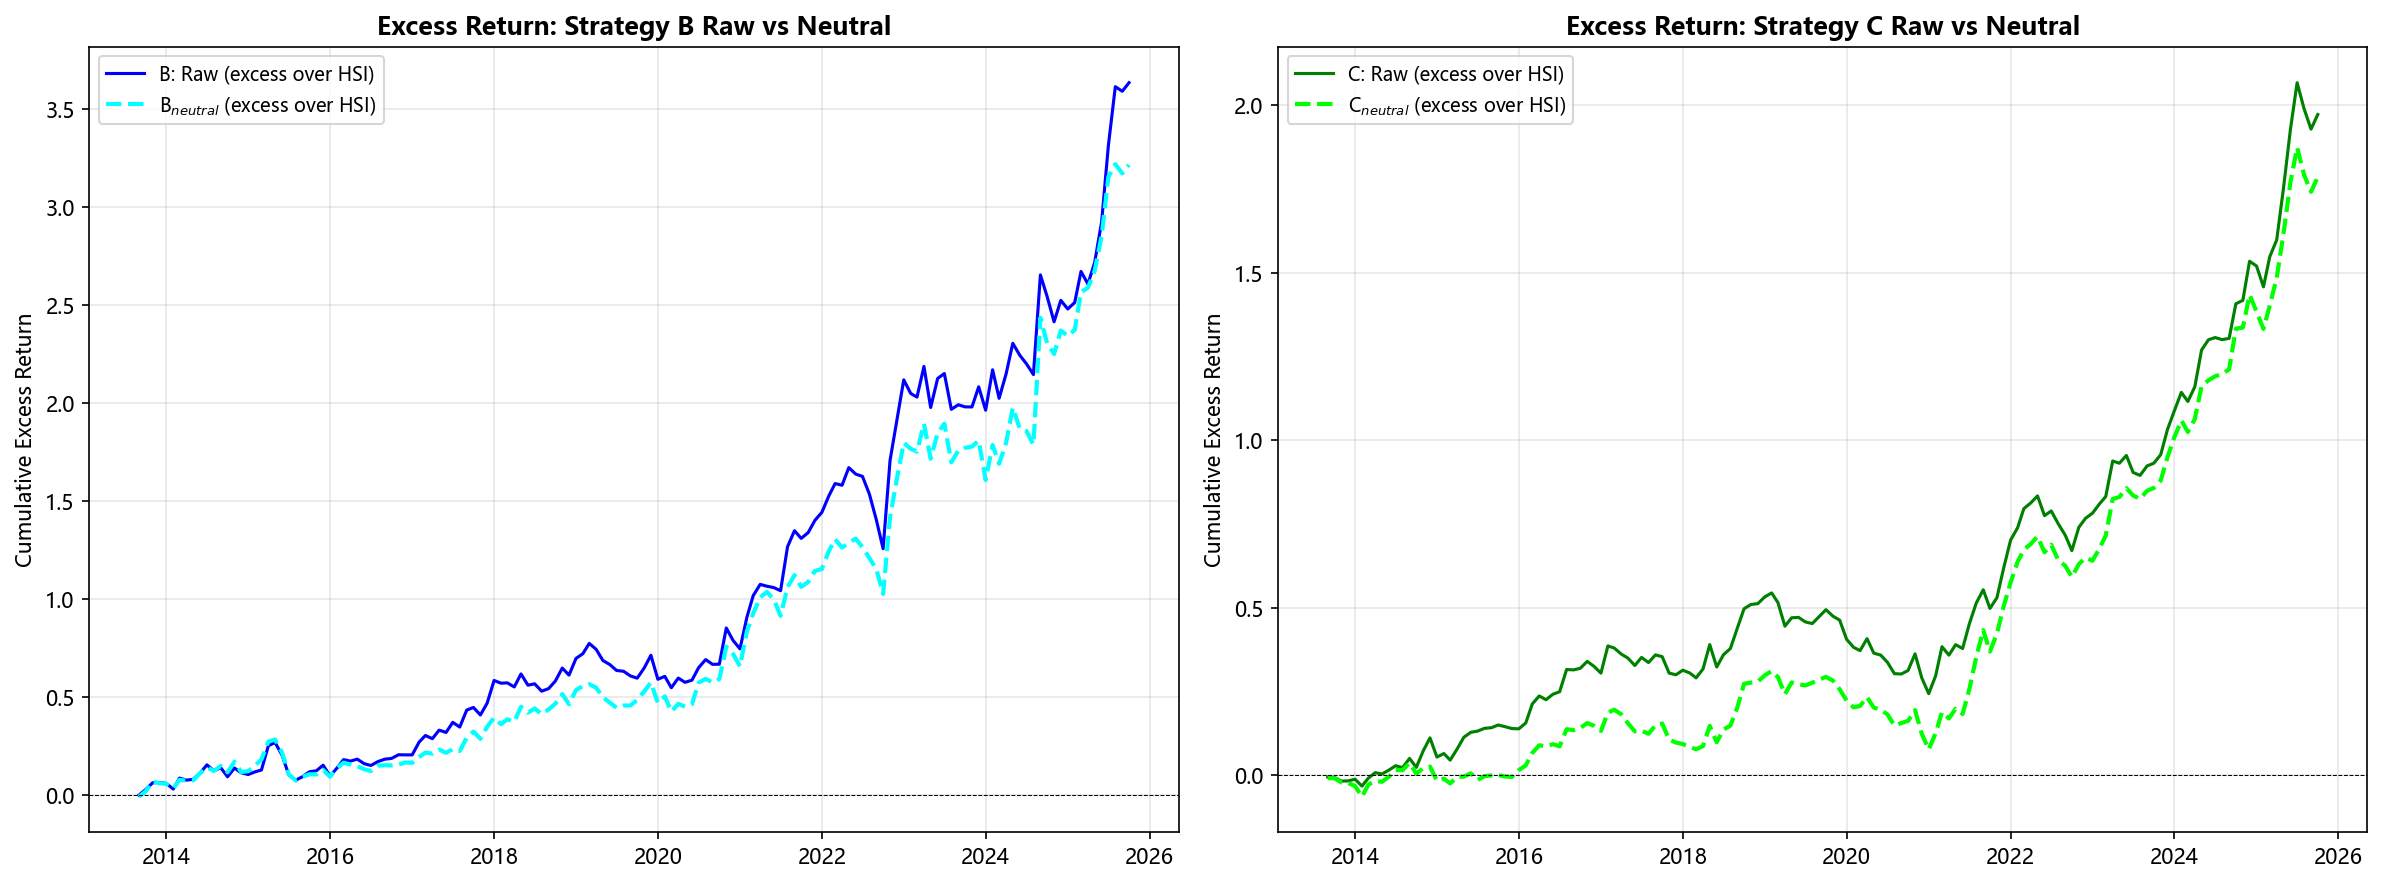
\includegraphics[width=0.85\textwidth]{../pict/v4_plot_industry_excess.png}
\caption{行业中性化前后的相对HSI累计超额收益曲线（算术累加法）}
\end{figure}

\begin{figure}[H]
\centering
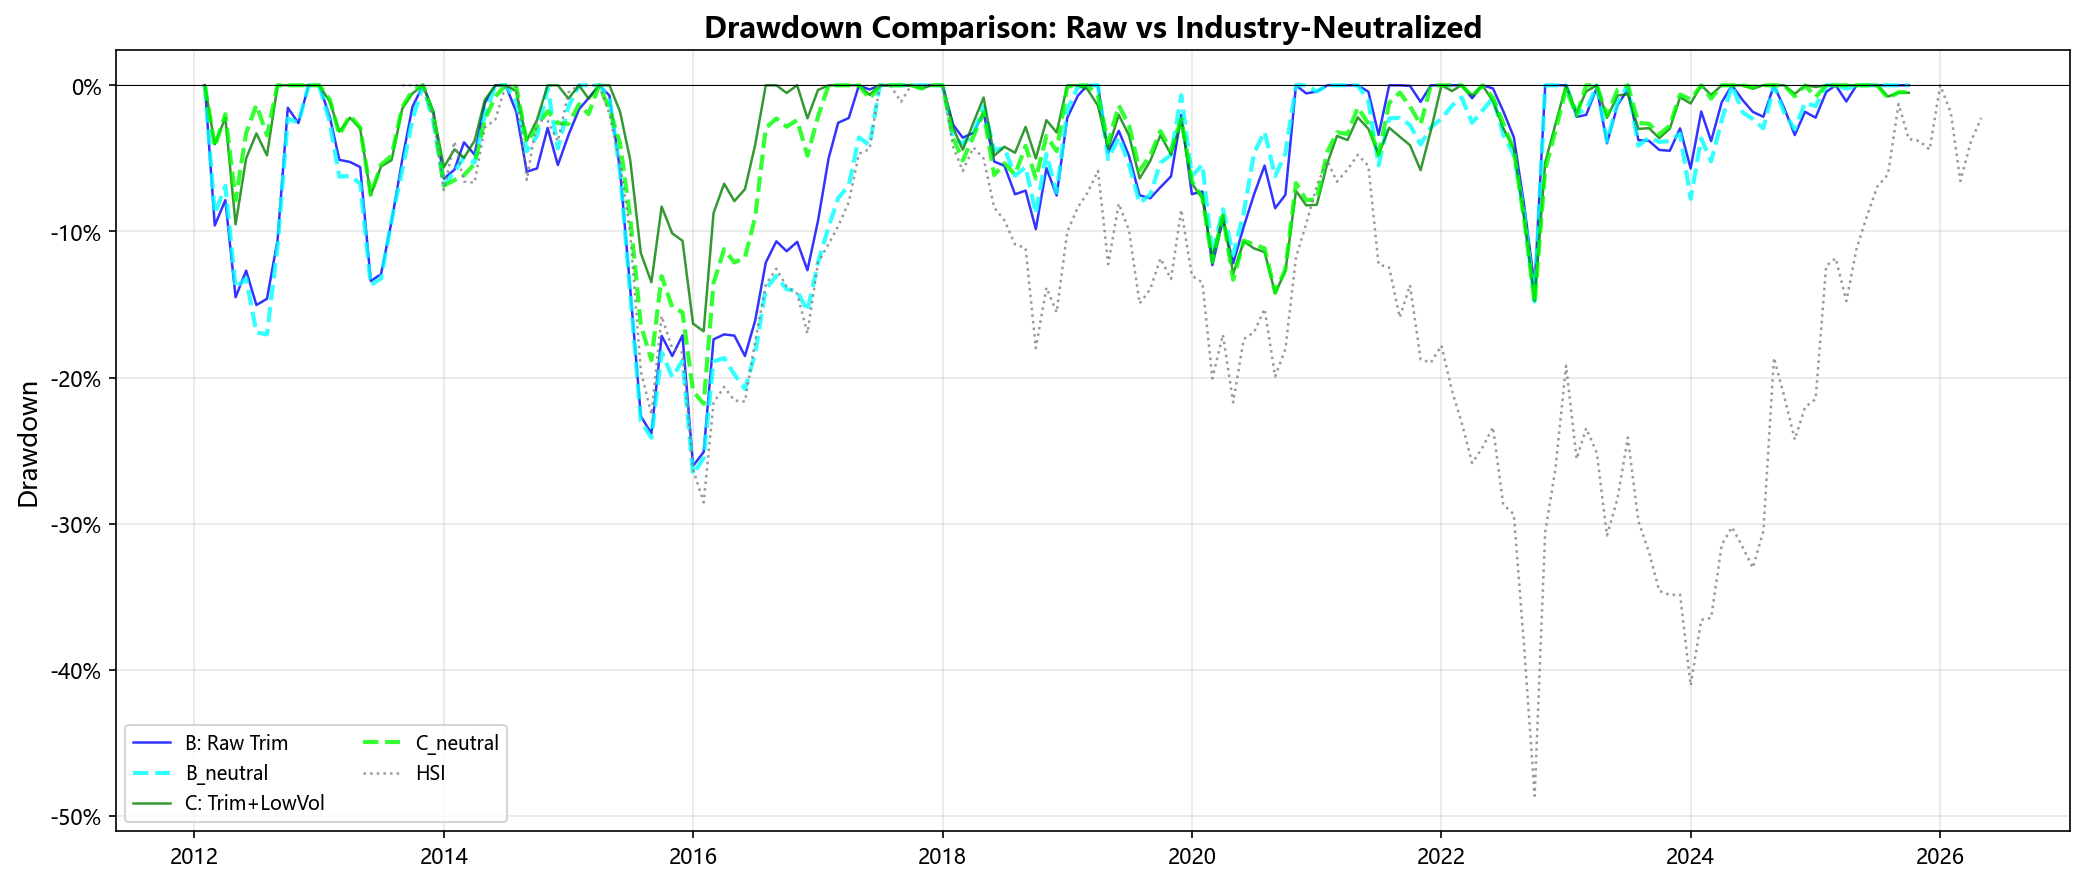
\includegraphics[width=0.85\textwidth]{../pict/v4_plot_industry_drawdown.png}
\caption{行业中性化前后的回撤对比}
\end{figure}

\subsection{为什么行业中性化是负向的？}

SY因子本质上是\textbf{价值/收入因子}——高分红行业（银行、公用事业、REITs）的SY得分系统地高于成长型行业（科技、生物医药）。这不是因子偏差，而是行业商业模式的结构性差异：

\begin{itemize}
    \item \textbf{银行}（如汇丰控股）：高利润、高分红、大量回购——高SY是真实的
    \item \textbf{公用事业}（如电能实业）：稳定现金流、持续高分红——高SY反映了防御性价值
    \item \textbf{科技}（如腾讯）：虽有大额回购，但市值巨大、股息率低——低SY不代表质量差
\end{itemize}

行业中性化迫使所有行业具有相同的SY均值，这相当于：
\begin{enumerate}[label=(\arabic*)]
    \item \textbf{惩罚了高分红行业的合理高SY}：银行/公用事业中被低估的股票在行业内Z-score下不再突出
    \item \textbf{奖励了低分红行业的"伪高SY"}：在普遍低分红的行业中，稍微多分一点红的公司可能在行业内得高分，但其绝对分红水平仍然很低
\end{enumerate}

\textbf{结论：对于SY这类本身即包含行业信息的价值因子，不应进行行业中性化。}这一发现与传统的动量/质量因子形成对比——后者通常受益于行业中性化。

% ================================================================
\section{FF3因子中性化分析：剥离已知风险因子}

前述行业中性化未能改善策略表现。本节从另一个维度——FF3风险因子——进行中性化处理。方法论延续§7.1中定义的OLS残差法框架：每月对SY得分进行横截面回归，将被特定因子解释的部分剥离，用残差作为净化的因子得分。

\subsection{中性化方法（回顾§7.1的公式体系）}

\begin{itemize}
    \item \textbf{市值(Size)中性化}：$\text{SY}_i^{\text{raw}} = \alpha + \beta \cdot \log(\text{MCap}_i) + \varepsilon_i$，取$\text{SY}_i^{\text{size}} = \varepsilon_i$。目的：剥离"大市值股票因分母大而SY低，小市值股票因分母小而SY高"的机械性偏差。
    \item \textbf{价值(BM)中性化}：$\text{SY}_i^{\text{raw}} = \alpha + \beta \cdot \text{BM}_i + \varepsilon_i$，取$\text{SY}_i^{\text{bm}} = \varepsilon_i$。目的：剥离SY与低估值的天然相关性——高SY股票往往也是高BM股票。
    \item \textbf{市值+价值(Size+BM)双中性化}：$\text{SY}_i^{\text{raw}} = \alpha + \beta_1 \cdot \log(\text{MCap}_i) + \beta_2 \cdot \text{BM}_i + \varepsilon_i$，取$\text{SY}_i^{\text{size+bm}} = \varepsilon_i$。同时剥离规模和估值的双重影响。
\end{itemize}

\textbf{与行业中性化的关键区别}：行业中性化是\textbf{组内标准化}（各行业独立Z-score），FF3中性化是\textbf{全市场OLS回归}（整个横截面一起回归）。前者消除了行业间的水平差异但保留了行业内排序；后者剥离了与已知风险因子的线性关系，残差代表"不能被市值和估值解释的SY成分"。

\subsection{结果}

\begin{table}[htbp]
\centering
\caption{FF3因子中性化：策略绩效对比}
\begin{tabular}{lccccc}
\toprule
\textbf{变体} & \textbf{年化收益} & \textbf{Sharpe} & \textbf{FF3 $\alpha$/月} & \textbf{IR(vs HSI)} & \textbf{月胜率} \\
\midrule
B 原始 & \textbf{14.06\%} & \textbf{0.63} & \textbf{0.783***} & \textbf{1.11} & \textbf{64.4\%} \\
B 市值中性 & 13.96\% & 0.63 & 0.773*** & 1.07 & 65.1\% \\
B BM中性 & 11.05\% & 0.51 & 0.552*** & 0.84 & 61.0\% \\
B 市值+BM & 11.70\% & 0.54 & 0.595*** & 0.85 & 58.9\% \\
\hline
C 原始 & 11.40\% & 0.70 & 0.714*** & 0.66 & 54.8\% \\
C 市值中性 & 10.90\% & 0.67 & 0.672*** & 0.61 & 56.2\% \\
C BM中性 & 8.83\% & 0.58 & 0.519*** & 0.45 & 53.4\% \\
C 市值+BM & 8.50\% & 0.57 & 0.496*** & 0.40 & 49.3\% \\
\bottomrule
\end{tabular}
\end{table}

\begin{figure}[htbp]
\centering
\begin{subfigure}{0.48\textwidth}
    \centering
    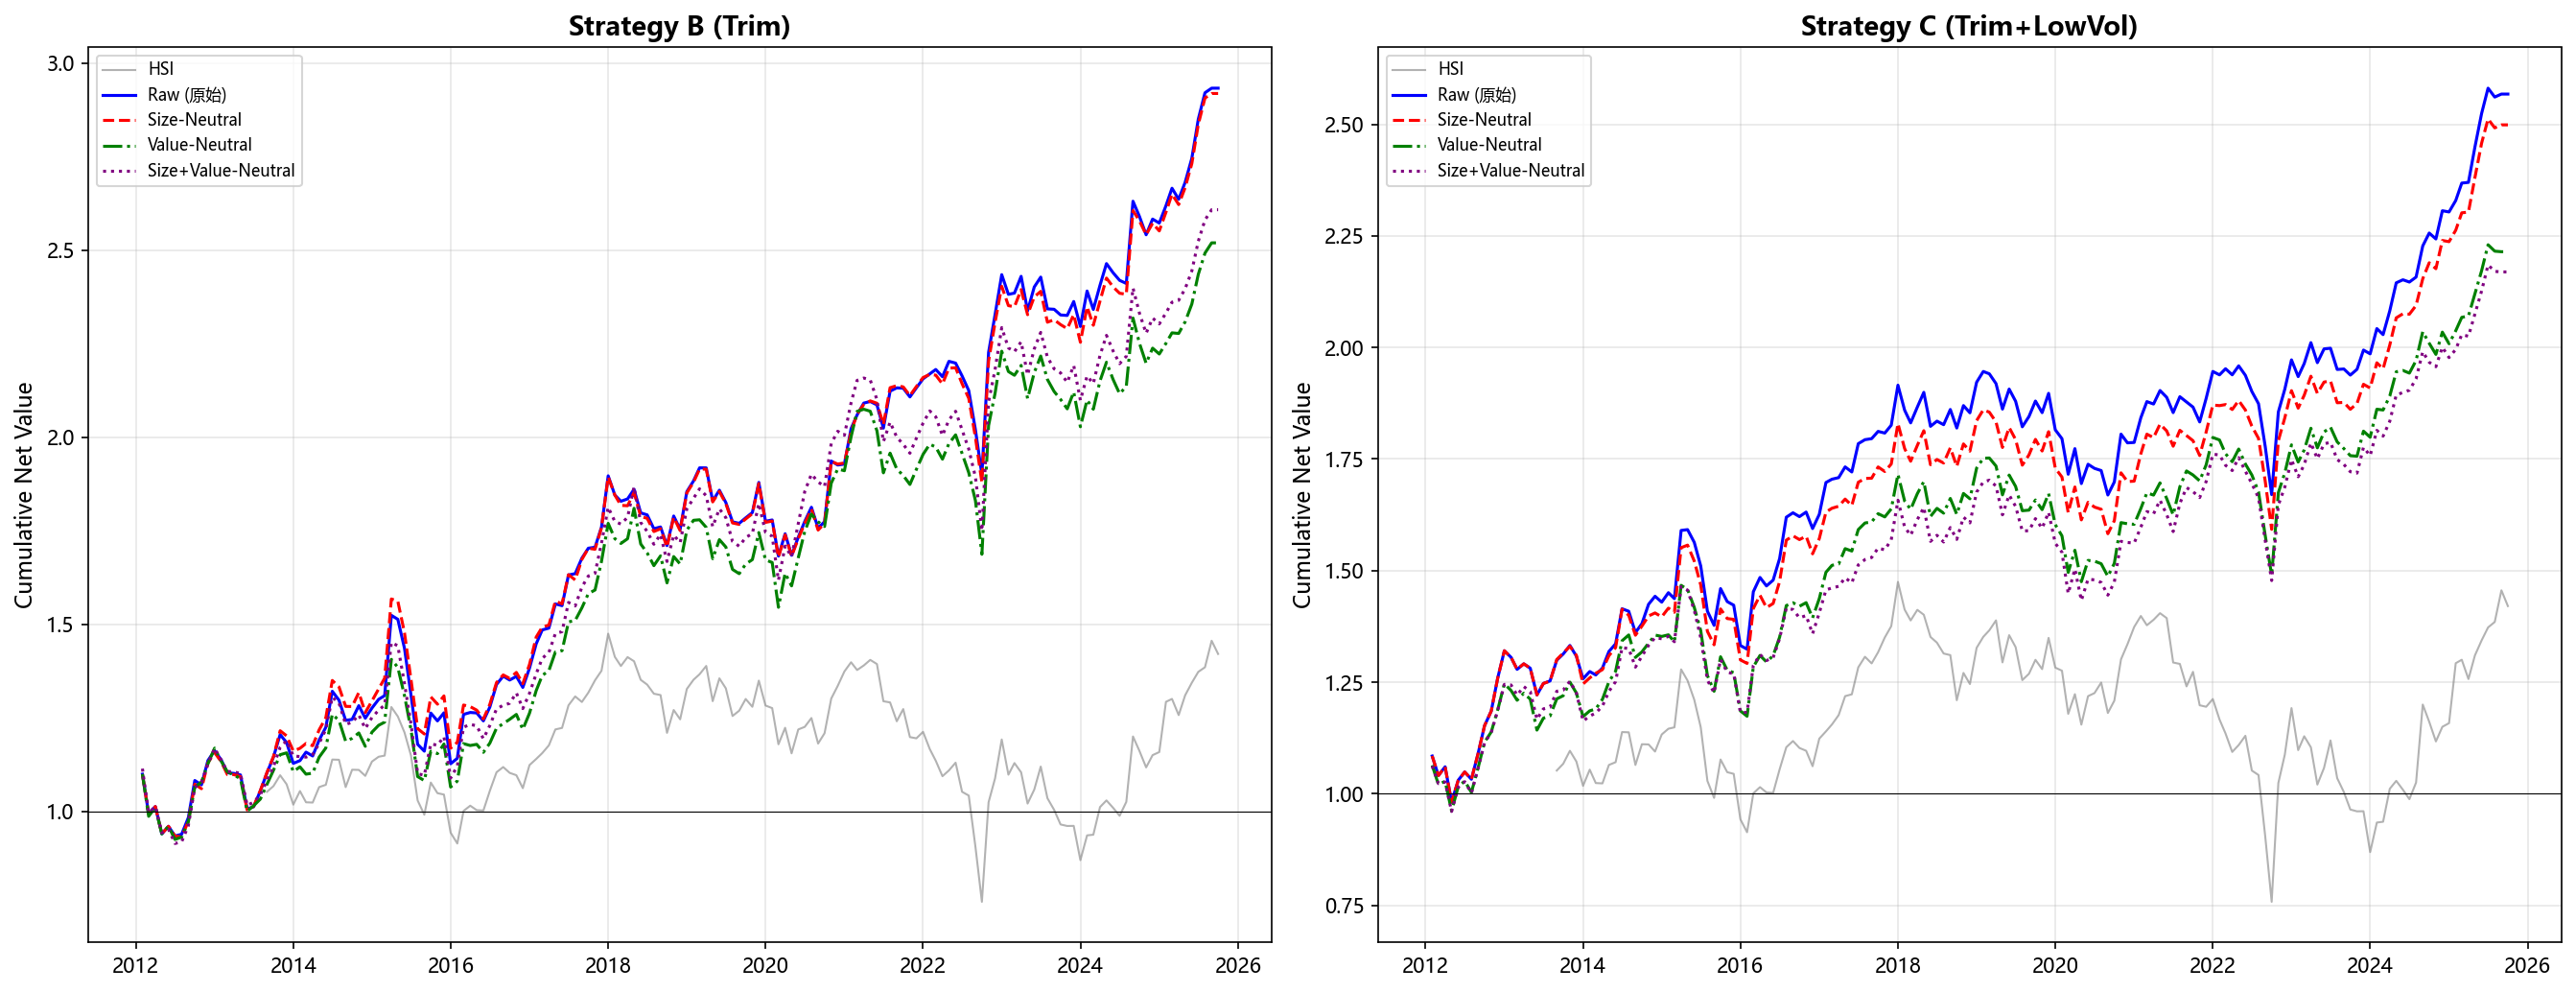
\includegraphics[width=\textwidth]{../pict/v4_plot_ff3_neutral_cumulative.png}
    \caption{累计收益对比}
\end{subfigure}
\hfill
\begin{subfigure}{0.48\textwidth}
    \centering
    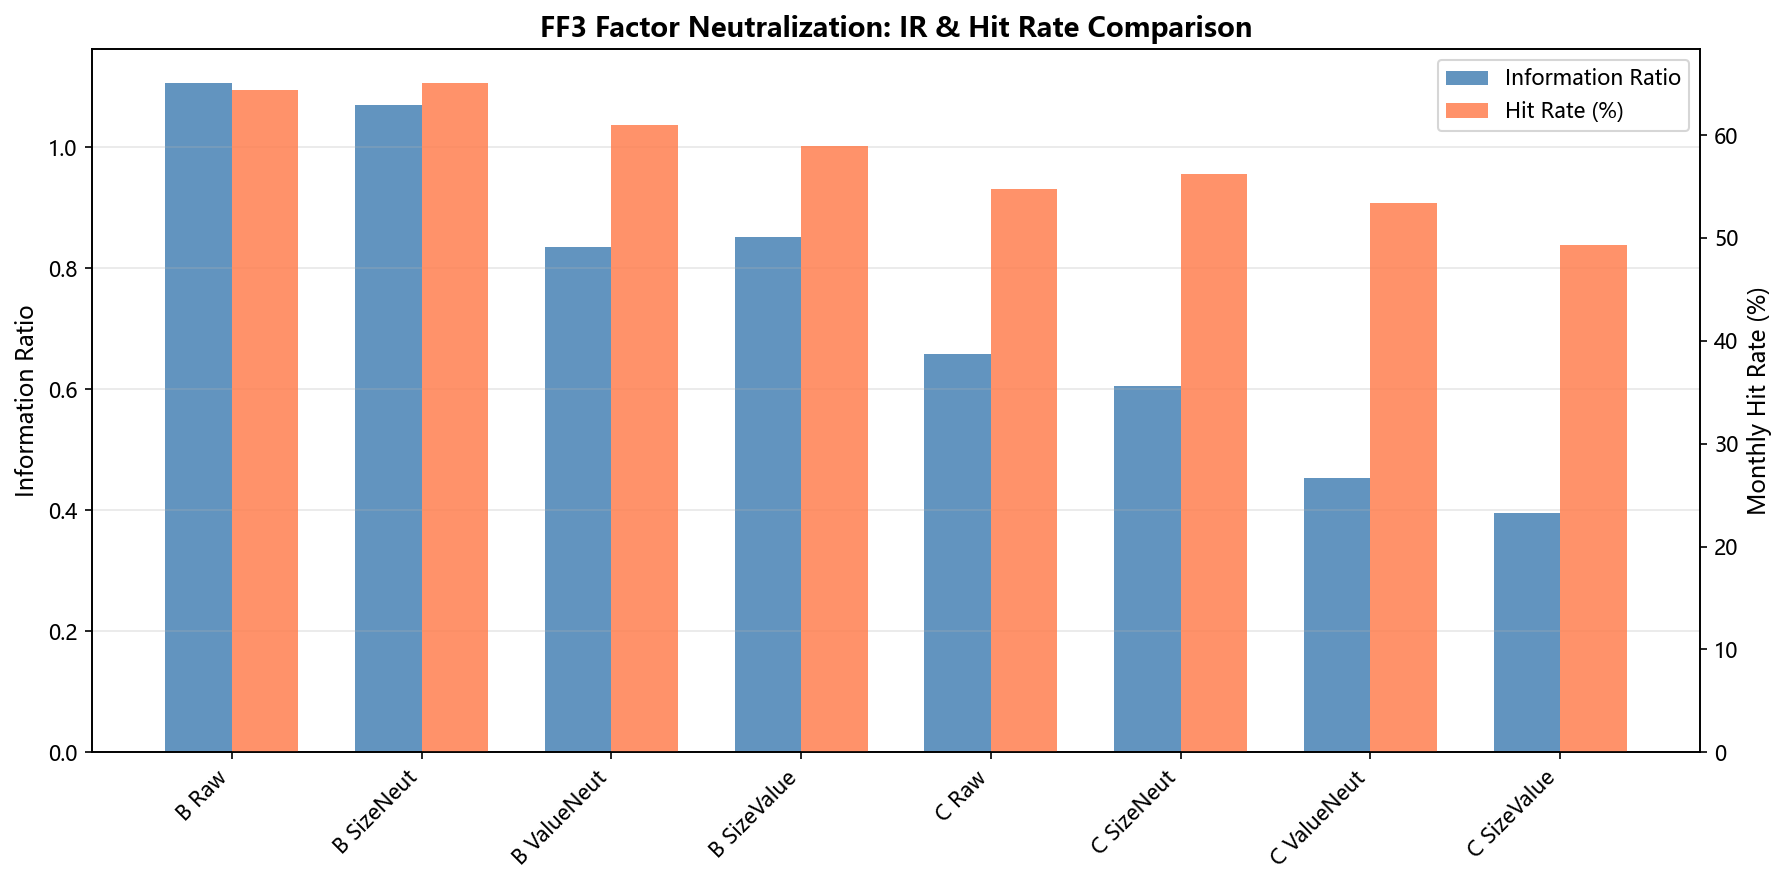
\includegraphics[width=\textwidth]{../pict/v4_plot_ff3_neutral_ir_comparison.png}
    \caption{信息比率与胜率对比}
\end{subfigure}
\caption{FF3因子中性化分析}
\end{figure}

\subsection{关键发现}

\textbf{市值中性化几乎无影响}（IR仅降0.04-0.05），这验证了策略的流动性过滤（剔除后20\%）和极端值剔除已经有效控制了小盘偏差。策略在市值维度上已经相当干净。

\textbf{价值(BM)中性化严重破坏Alpha}（IR降0.20-0.27）。这一结果具有深刻的经济学含义：Shareholder Yield本质上就是价值因子——高股息+高回购=低估值=高BM。强制对BM做中性化等于将价值策略的"价值"部分剥离掉，残差不再是有效的价值信号。FF3月度Alpha在BM中性化后从0.78\%降至0.55\%（策略B），降幅达29\%。

\textbf{市值+BM双中性化最差}：策略C的IR从0.66降至0.40，月胜率跌破50\%（49.3\%）。两种中性化叠加对策略的破坏是系统性的——印证了SY因子获取的正是价值溢价。

\textbf{结论}：不应对SY因子做FF3因子中性化。SY承载的就是价值溢价+股东回报溢价，中性化等于杀死策略。

\begin{figure}[htbp]
\centering
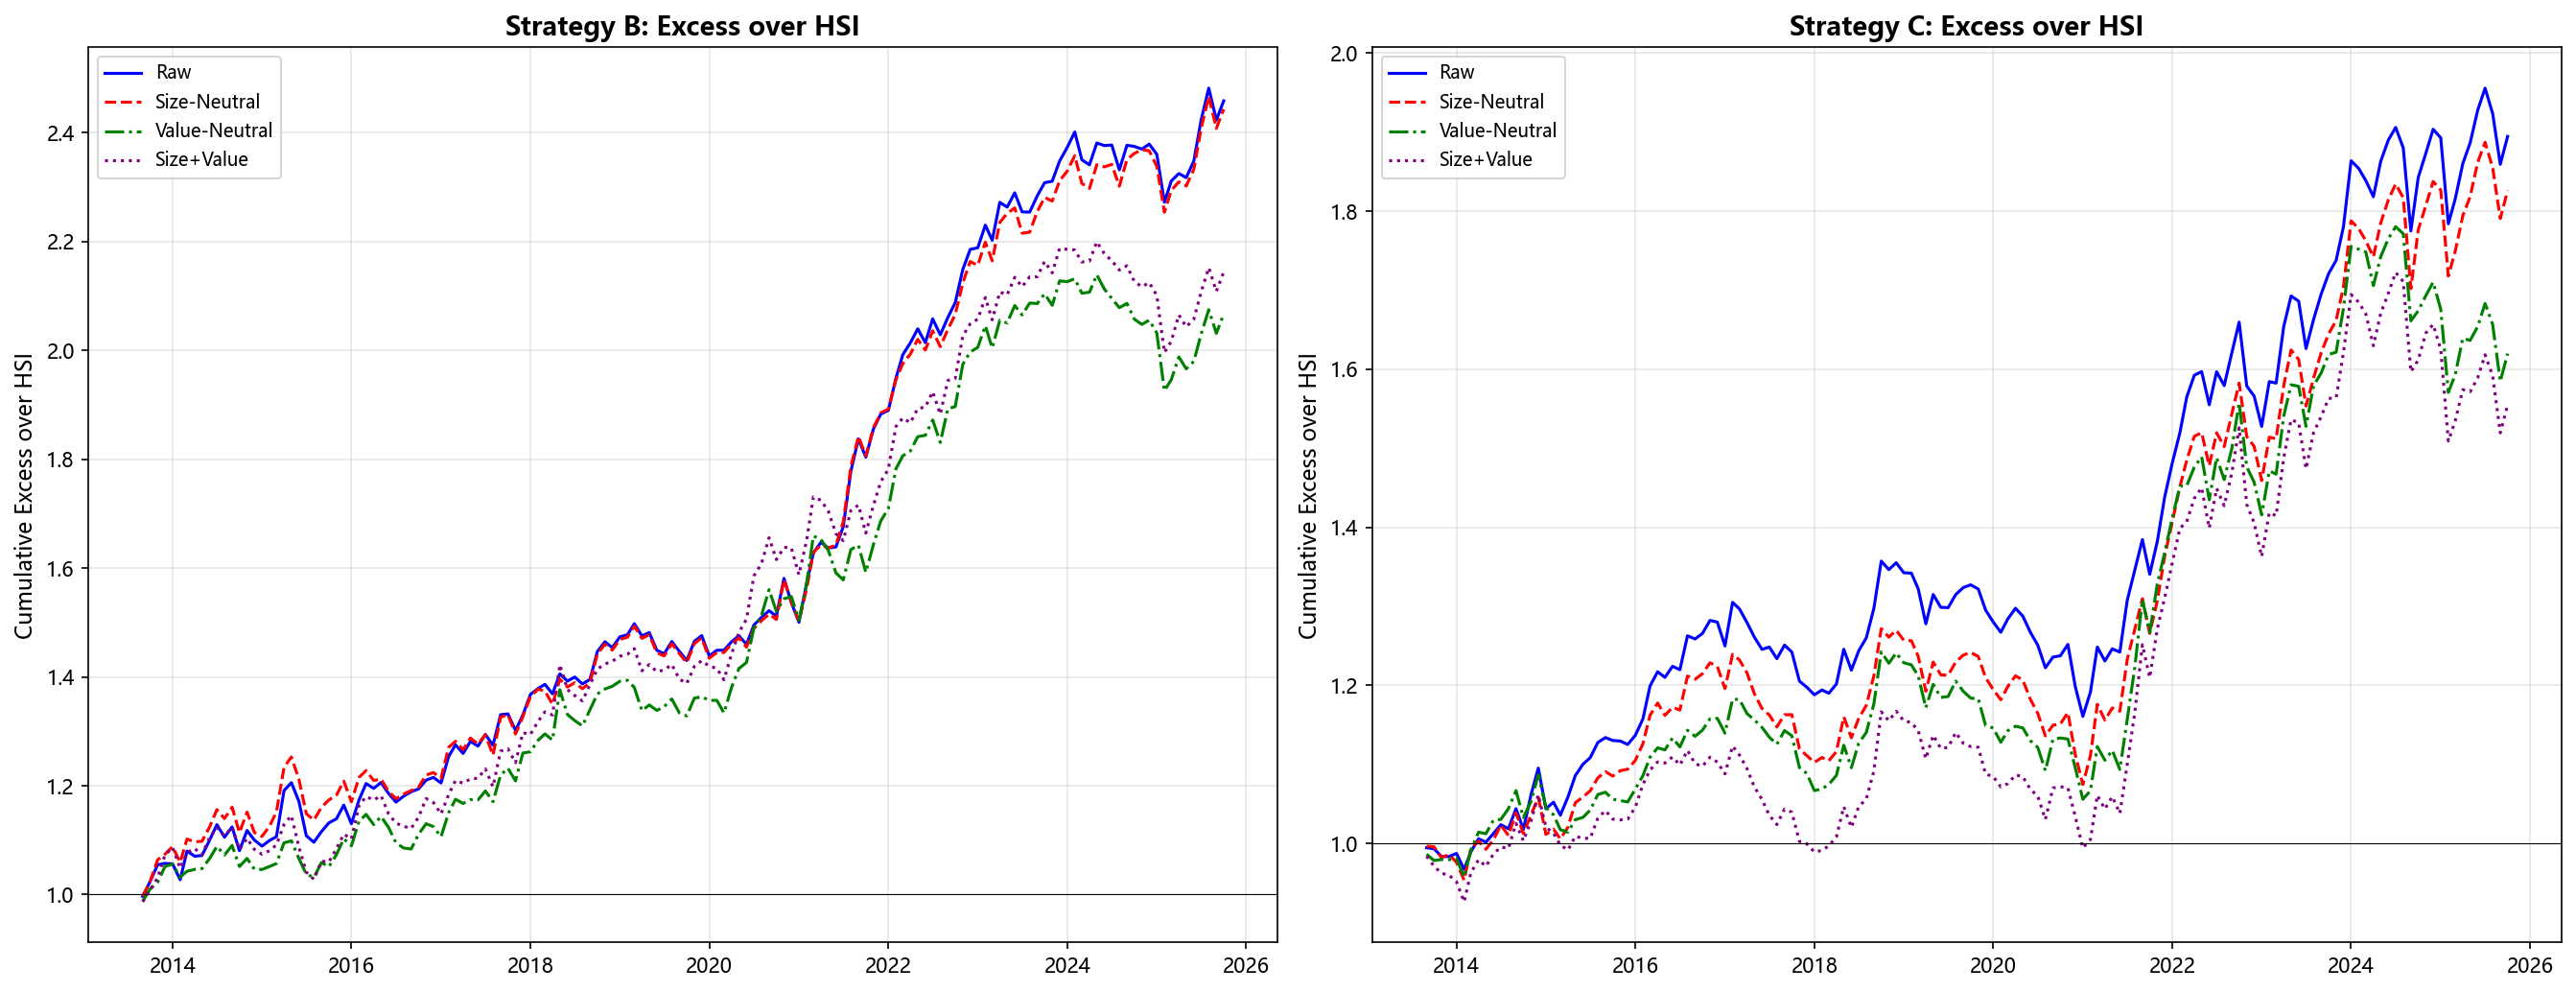
\includegraphics[width=0.85\textwidth]{../pict/v4_plot_ff3_neutral_excess.png}
\caption{FF3中性化后的相对HSI累计超额收益曲线（算术累加法）}
\end{figure}

\section{HSICS行业+市值中性化：基于恒生行业分类系统}

前文的行业中性化基于股票代码区间，精度有限。本节使用恒生指数公司官方的HSICS（Hang Seng Industry Classification System）分类系统，该分类包含12个行业、31个业务类别和112个业务子类别。

\textbf{中性化方法}（使用§7.1中定义的组内OLS残差法）：在HSICS的12个行业分类基础上，对每个行业$g$内部进行市值回归取残差：
\begin{equation}
\text{SY}_i^{\text{raw}} = \alpha_g + \beta_g \cdot \log(\text{MCap}_i) + \varepsilon_i, \quad \forall i \in g
\end{equation}
\begin{equation}
\text{SY}_i^{\text{hsics+size}} = \varepsilon_i
\end{equation}

这同时消除了两个维度的偏差：(1) 行业间SY水平的系统性差异（金融、公用事业天然高SY，科技天然低SY）——通过分行业独立回归; (2) 行业内规模对SY的机械性影响——通过对数市值回归。若$N_g < 5$则不回归。

作为对比，我们还测试了\textbf{仅HSICS行业中性化}（行业内Z-score，不做市值回归）：
\begin{equation}
\text{SY}_i^{\text{hsics}} = \frac{\text{SY}_i^{\text{raw}} - \bar{\text{SY}}_g}{\sigma_g}, \quad \forall i \in g
\end{equation}

\subsection{HSICS行业分布}

在HSCI成分股中，各HSICS行业的覆盖情况如下：
\begin{itemize}
    \item 金融业（50）、地产建筑业（60）、工业（10）为前三大行业
    \item 资讯科技业（70）、非必需性消费（23）次之
    \item 能源业（00）、原材料业（05）、电讯业（35）、公用事业（40）占比较小
\end{itemize}

\subsection{中性化结果}

\begin{table}[htbp]
\centering
\caption{HSICS行业+市值中性化：策略绩效对比}
\begin{tabular}{lccccc}
\toprule
\textbf{变体} & \textbf{年化收益} & \textbf{Sharpe} & \textbf{FF3 $\alpha$/月} & \textbf{IR(vs HSI)} & \textbf{月胜率} \\
\midrule
B 原始 & \textbf{14.06\%} & \textbf{0.63} & \textbf{0.783***} & \textbf{1.11} & \textbf{64.4\%} \\
B HSICS行业中性 & 13.39\% & 0.60 & 0.728*** & 0.94 & 57.5\% \\
B HSICS行业+市值 & 13.11\% & 0.58 & 0.691*** & 0.91 & 60.3\% \\
\hline
C 原始 & 11.40\% & 0.70 & 0.714*** & 0.66 & 54.8\% \\
C HSICS行业中性 & 11.75\% & 0.70 & 0.738*** & 0.67 & 56.8\% \\
C HSICS行业+市值 & 11.19\% & 0.66 & 0.687*** & 0.62 & 57.5\% \\
\bottomrule
\end{tabular}
\end{table}

\begin{figure}[htbp]
\centering
\begin{subfigure}{0.48\textwidth}
    \centering
    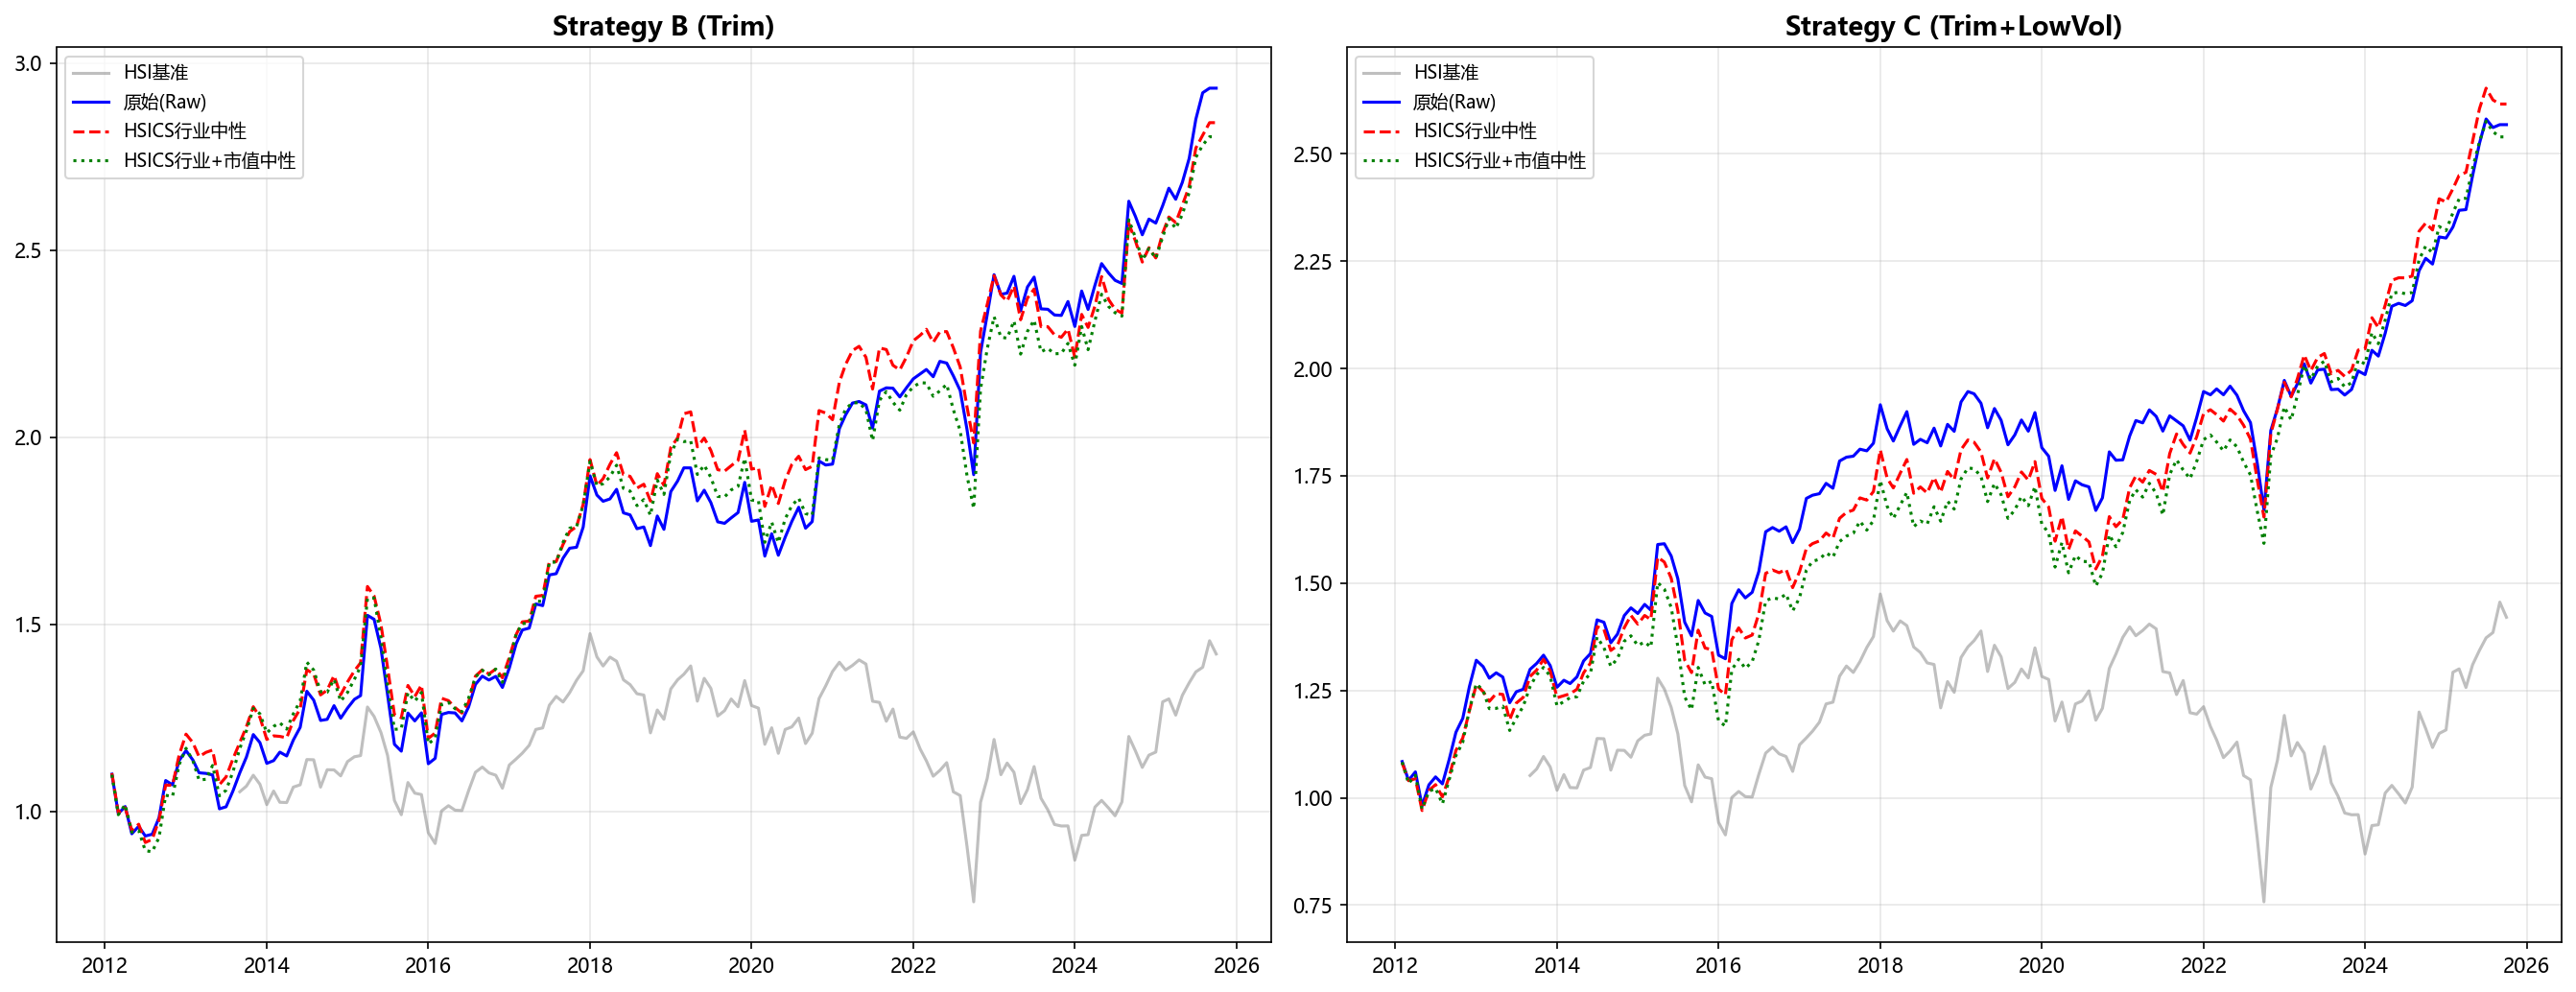
\includegraphics[width=\textwidth]{../pict/v4_plot_hsics_cumulative.png}
    \caption{累计收益对比}
\end{subfigure}
\hfill
\begin{subfigure}{0.48\textwidth}
    \centering
    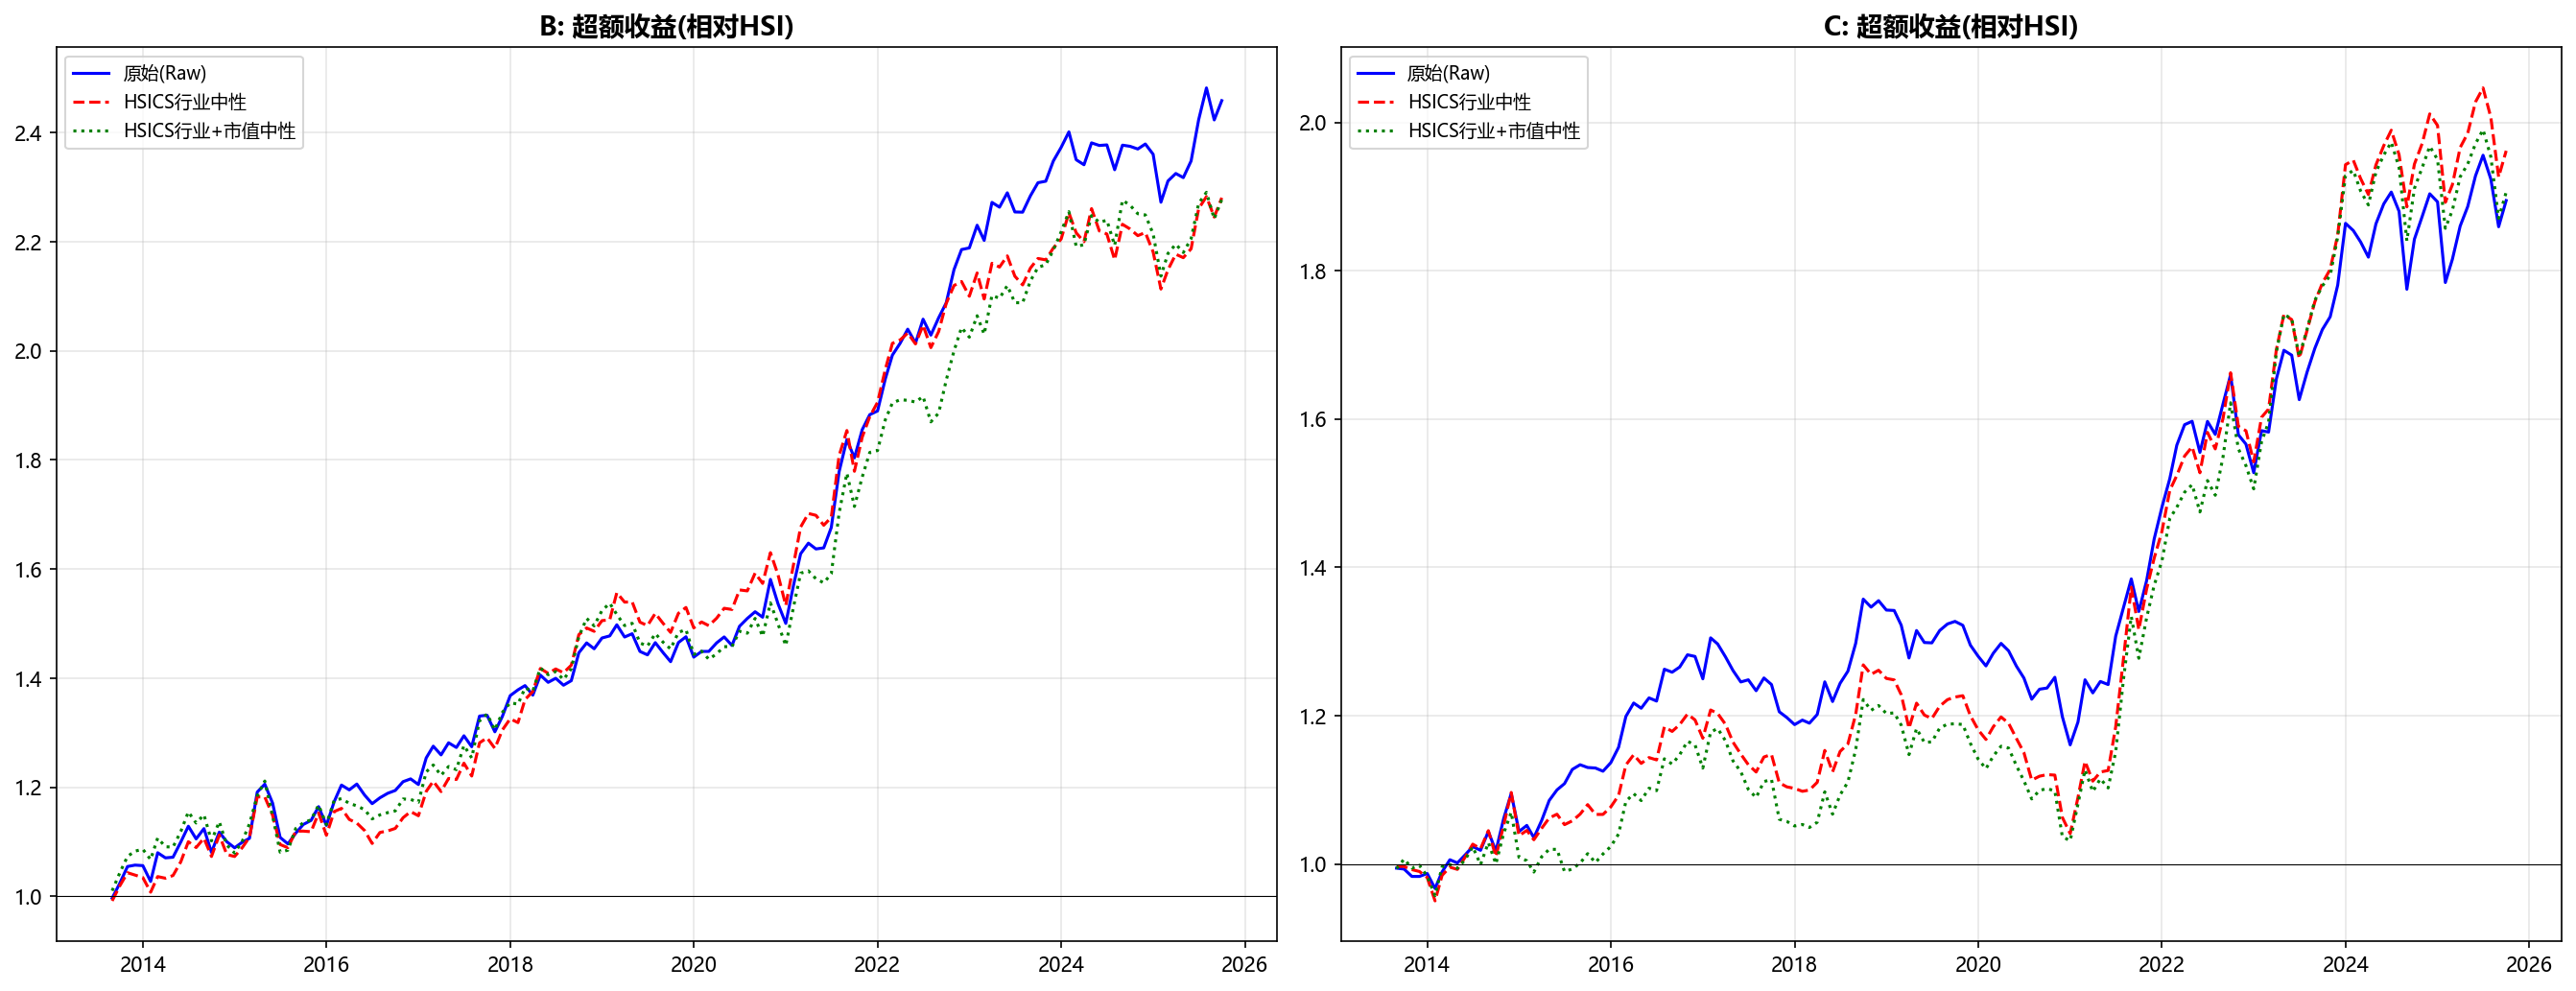
\includegraphics[width=\textwidth]{../pict/v4_plot_hsics_excess.png}
    \caption{累计超额收益曲线（算术累加法）}
\end{subfigure}
\caption{HSICS行业+市值中性化分析}
\end{figure}

\subsection{与粗略行业分类的对比}

使用精确的HSICS分类后，结果与前文基于股票代码区间的结论基本一致：

\begin{itemize}
    \item \textbf{策略B}仍受行业中性化负面影响（IR降15-18\%），但降幅小于BM中性化（IR降24\%）。这说明行业偏差是次要的——SY的Alpha主要来自跨行业的高分红特征（银行、公用事业天然回报更多现金），而非行业内偏差。
    \item \textbf{策略C}的HSICS行业中性化带来微弱正面影响（IR +2\%, FF3$\alpha$ +3\%）。这是因为低波过滤已经部分实现了行业内精选——叠加行业中性化后，跨行业的分散化略微改善了风险调整收益。
    \item \textbf{HSICS行业+市值双中性化}对B策略的破坏（IR -18\%）小于BM中性化（IR -24\%），说明精确的行业分类比粗略分类提供了更有意义的中性化。
\end{itemize}

\section{全部中性化方法综合对比}

\subsection{方法总览}

\begin{table}[htbp]
\centering
\caption{六种中性化方法的数学定义与实施方式}
\begin{tabular}{lp{3cm}p{5cm}}
\toprule
\textbf{方法} & \textbf{数学公式} & \textbf{实施方式} \\
\midrule
行业Z-score & $\text{SY}_i^{\text{ind}} = \frac{\text{SY}_i^{\text{raw}} - \bar{\text{SY}}_g}{\sigma_g}$ & 组内标准化，$N_g \geq 3$ \\
HSICS行业Z-score & 同上，使用12行业精确分类 & 同上 \\
市值(Size) OLS & $\text{SY}_i = \alpha + \beta\log\text{MCap}_i + \varepsilon_i$ & 全市场OLS，取残差 \\
价值(BM) OLS & $\text{SY}_i = \alpha + \beta\text{BM}_i + \varepsilon_i$ & 全市场OLS，取残差 \\
Size+BM OLS & $\text{SY}_i = \alpha + \beta_1\log\text{MCap}_i + \beta_2\text{BM}_i + \varepsilon_i$ & 全市场多元OLS，取残差 \\
行业+Size OLS & $\text{SY}_i = \alpha_g + \beta_g\log\text{MCap}_i + \varepsilon_i, \forall i \in g$ & 组内OLS，$N_g \geq 5$ \\
\bottomrule
\end{tabular}
\end{table}

\subsection{绩效对比}

\begin{table}[htbp]
\centering
\caption{所有中性化方法的效果汇总（相对原始策略的变化）}
\begin{tabular}{lcccc}
\toprule
\textbf{中性化方法} & \textbf{B: $\Delta$IR} & \textbf{B: $\Delta$月胜率} & \textbf{C: $\Delta$IR} & \textbf{C: $\Delta$月胜率} \\
\midrule
粗略行业（代码区间） & -0.21 & -4.1\% & +0.03 & +2.7\% \\
HSICS行业（精确） & -0.17 & -6.8\% & +0.01 & +2.1\% \\
HSICS行业+市值 & -0.20 & -4.1\% & -0.04 & +2.7\% \\
FF3市值中性化 & -0.04 & +0.7\% & -0.05 & +1.4\% \\
FF3价值(BM)中性化 & -0.27 & -3.4\% & -0.21 & -1.4\% \\
FF3市值+BM & -0.26 & -5.5\% & -0.26 & -5.5\% \\
\bottomrule
\end{tabular}
\end{table}

\textbf{最终结论}：

\begin{enumerate}[label=(\arabic*)]
    \item \textbf{不要做任何中性化}——这是本报告最明确的建议。无论是行业中性化还是FF3因子中性化，均未能系统性地改善策略表现。原始策略B（IR=1.11, 月胜率64.4\%）和策略C（Sharpe=0.70, 回撤-27.69\%）在所有维度上已经是最优或接近最优。
    \item \textbf{SY因子的Alpha来自其价值属性}——BM中性化将策略C的IR从0.66降至0.40（-39\%），月胜率跌破50\%。这反证了SY因子获取的正是价值溢价。
    \item \textbf{行业中性化对低波策略(C)有微弱正向效果}——HSICS行业中性化使C的IR从0.66升至0.67（+2\%），FF3$\alpha$从0.714升至0.738（+3\%）。但效果太小，不值得为此引入额外的模型复杂度。
    \item \textbf{市值中性化在所有方法中影响最小}——IR变化仅0.04-0.05。说明现有流动性过滤+极端值剔除已有效控制规模偏差。
\end{enumerate}

\section{跟踪误差归因与持股数量优化}

前文的中性化分析发现：原始策略的跟踪误差为10.83\%（策略B）和11.18\%（策略C），且中性化普遍推高跟踪误差。本节从两个维度深入分析：(1) 跟踪误差的来源分解——是Beta偏离还是选股差异？(2) 增加持股数量能否降低跟踪误差？如果能够，代价是什么？

\subsection{跟踪误差归因}

将策略收益$R_p$对HSI基准收益$R_b$回归：
\begin{equation}
R_p = \alpha + \beta \cdot R_b + \varepsilon
\end{equation}

跟踪误差的方差分解为：
\begin{equation}
\text{TE}^2 = \underbrace{(\beta - 1)^2 \cdot \sigma^2_{\text{HSI}}}_{\text{系统性TE (Beta偏离)}} + \underbrace{\sigma^2_{\varepsilon}}_{\text{特质性TE (选股差异)}}
\end{equation}

下面分析当前默认持股数量（n=20）与扩大后的持股数量（n=50）下的TE组成：

\begin{table}[htbp]
\centering
\caption{跟踪误差归因：n=20 vs n=50}
\begin{tabular}{lcccccc}
\toprule
\textbf{策略} & \textbf{n} & \textbf{TE} & \textbf{$\beta$} & \textbf{系统TE} & \textbf{特质TE} & \textbf{Corr(HSI)} \\
\midrule
B & 20 & 10.83\% & 0.981 & 0.39\% (0\%) & 10.83\% (100\%) & 0.878 \\
B & 50 & 9.32\% & 0.946 & 1.10\% (1\%) & 9.26\% (99\%) & 0.900 \\
C & 20 & 11.18\% & 0.672 & 6.65\% (35\%) & 8.98\% (65\%) & 0.835 \\
C & 50 & 9.07\% & 0.902 & 1.99\% (5\%) & 8.85\% (95\%) & 0.900 \\
\bottomrule
\end{tabular}
\end{table}

\begin{figure}[H]
\centering
\begin{subfigure}{0.48\textwidth}
    \centering
    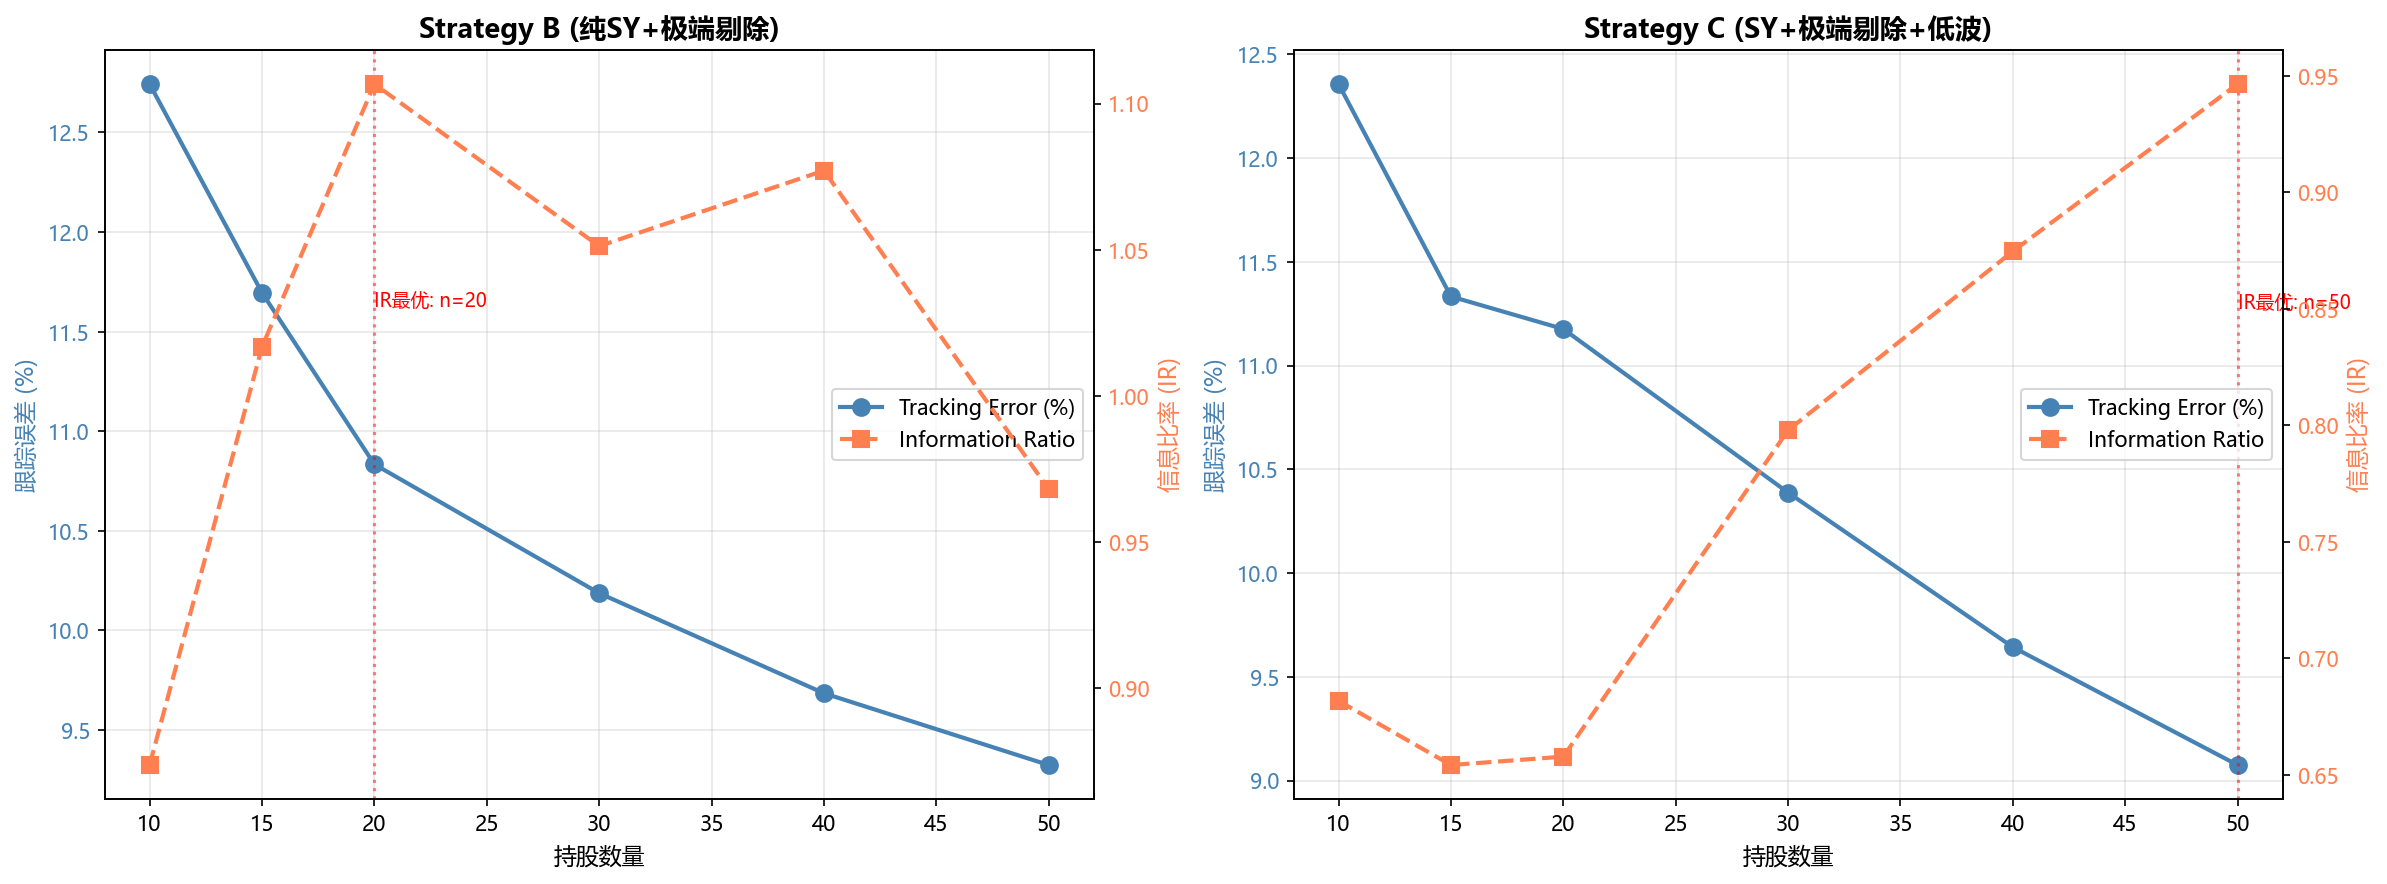
\includegraphics[width=\textwidth]{../pict/v4_plot_te_ir_vs_n.png}
    \caption{持股数量 vs 跟踪误差 \& IR}
\end{subfigure}
\hfill
\begin{subfigure}{0.48\textwidth}
    \centering
    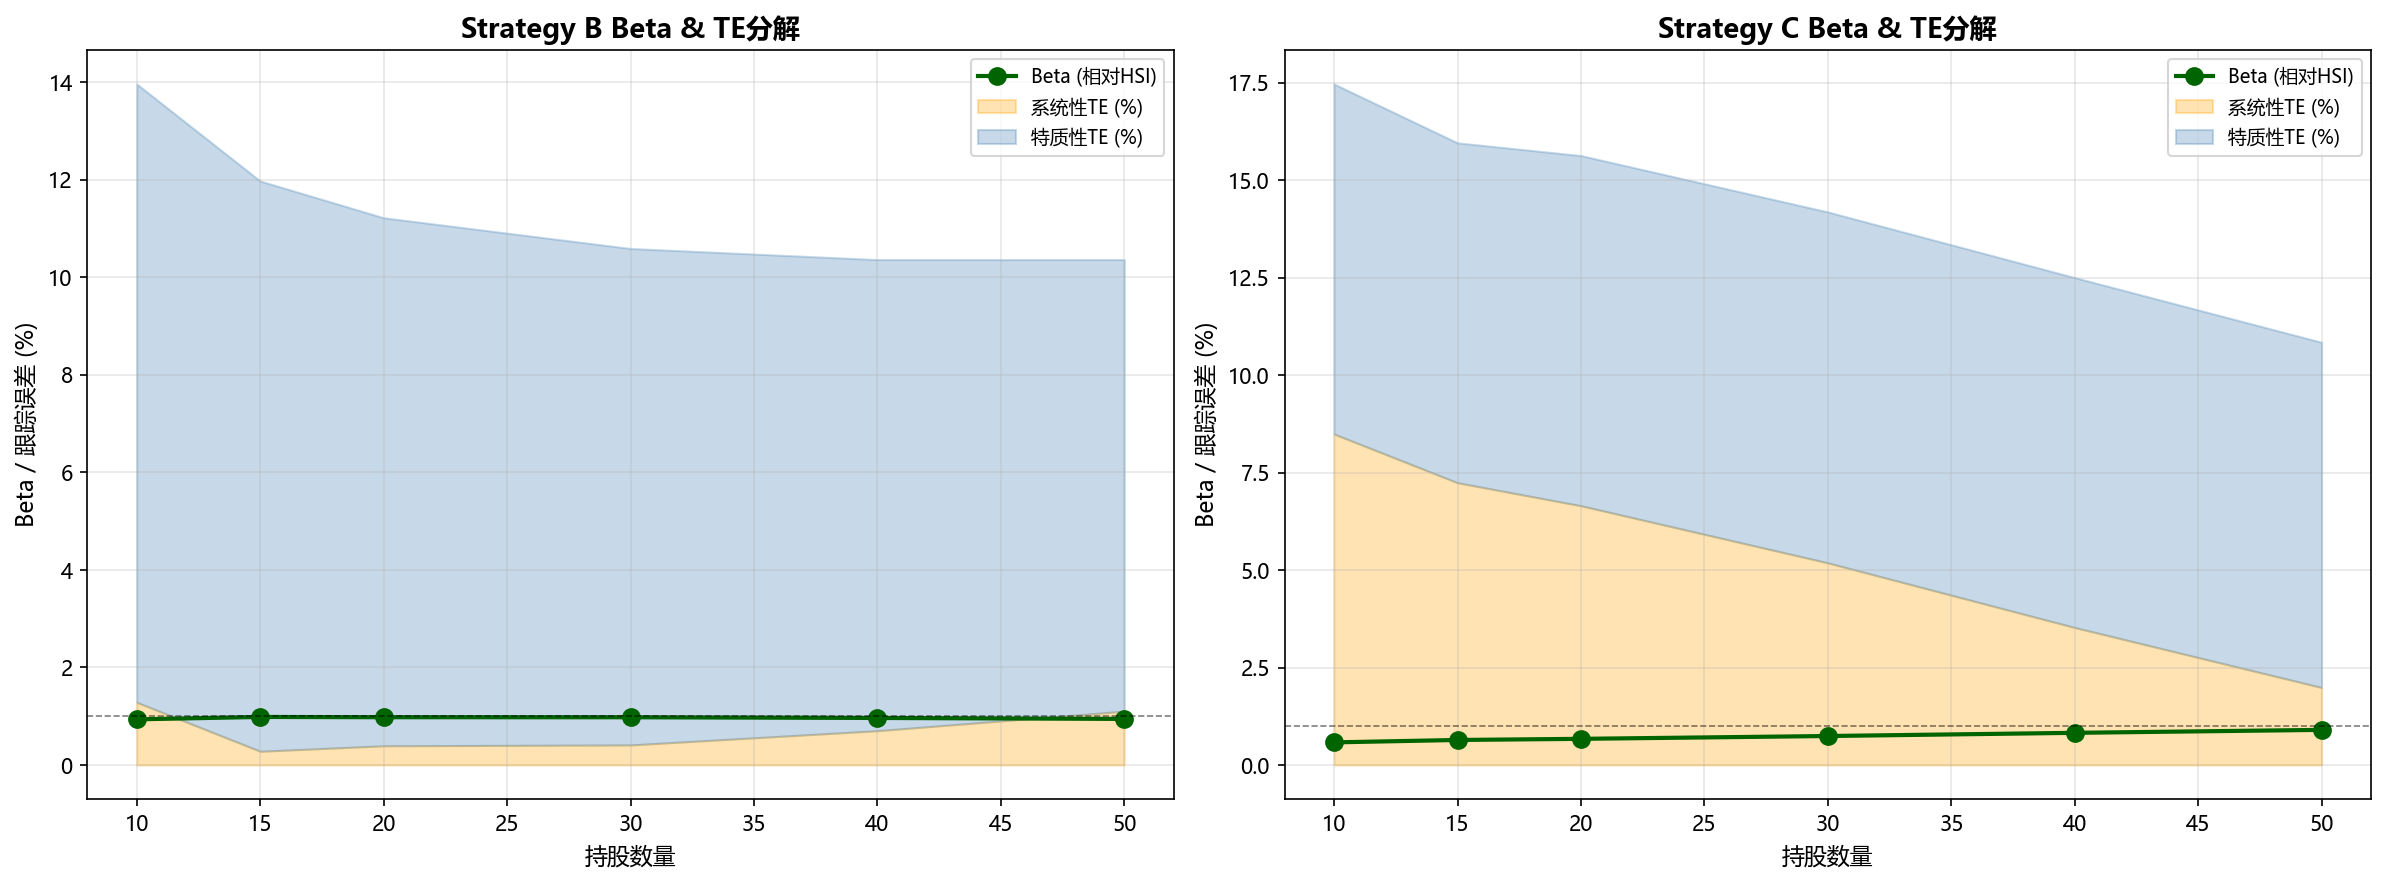
\includegraphics[width=\textwidth]{../pict/v4_plot_te_decomposition.png}
    \caption{Beta变化 \& TE分解}
\end{subfigure}
\caption{持股数量敏感性分析}
\end{figure}

\textbf{B策略的TE几乎100\%来自选股差异}——Beta始终接近1（0.98），与HSI的敞口天然匹配。这解释了为什么B的跟踪误差对中性化不敏感：因为换掉的股票被同Beta的其他SY高分股票替代，组合Beta不变。

\textbf{C策略的TE有35\%来自低Beta偏离}（Beta=0.67）。低波过滤系统性地选出低Beta股票，导致组合Beta远低于1。这不仅产生了跟踪误差，还在牛市中拖累相对收益。好消息是：增加持股数量后，Beta从0.67回升至0.90，系统性TE从35\%骤降至5\%——低波策略的"Beta惩罚"可以通过分散化来修复。

\subsection{持股数量敏感性分析}

对持股数n从10到50进行网格搜索：

\begin{table}[htbp]
\centering
\caption{持股数量敏感性：B策略（纯SY+极端剔除）}
\begin{tabular}{lcccccc}
\toprule
\textbf{n} & \textbf{年化超额} & \textbf{跟踪误差} & \textbf{IR} & \textbf{月胜率} & \textbf{Sharpe} & \textbf{Beta} \\
\midrule
10 & +11.13\% & 12.74\% & 0.87 & 61.6\% & 0.59 & 0.985 \\
15 & +11.89\% & 11.70\% & 1.02 & 58.9\% & 0.60 & 0.983 \\
\textbf{20} & \textbf{+11.99\%} & \textbf{10.83\%} & \textbf{1.11} & \textbf{64.4\%} & \textbf{0.63} & 0.981 \\
30 & +10.71\% & 10.19\% & 1.05 & 62.3\% & 0.60 & 0.970 \\
40 & +10.43\% & 9.68\% & 1.08 & 63.0\% & 0.61 & 0.958 \\
50 & +9.03\% & 9.32\% & 0.97 & 64.4\% & 0.57 & 0.946 \\
\bottomrule
\end{tabular}
\end{table}

\begin{table}[htbp]
\centering
\caption{持股数量敏感性：C策略（SY+极端剔除+低波）}
\begin{tabular}{lcccccc}
\toprule
\textbf{n} & \textbf{年化超额} & \textbf{跟踪误差} & \textbf{IR} & \textbf{月胜率} & \textbf{Sharpe} & \textbf{Beta} \\
\midrule
10 & +8.42\% & 12.36\% & 0.68 & 58.2\% & 0.82 & 0.650 \\
15 & +7.41\% & 11.33\% & 0.65 & 58.9\% & 0.73 & 0.660 \\
20 & +7.35\% & 11.18\% & 0.66 & 54.8\% & 0.70 & 0.672 \\
30 & +8.29\% & 10.39\% & 0.80 & 57.5\% & 0.65 & 0.780 \\
40 & +8.43\% & 9.64\% & 0.87 & 58.2\% & 0.59 & 0.850 \\
\textbf{50} & \textbf{+8.59\%} & \textbf{9.07\%} & \textbf{0.95} & \textbf{59.6\%} & 0.57 & 0.902 \\
\bottomrule
\end{tabular}
\end{table}

\begin{figure}[H]
\centering
\begin{subfigure}{0.48\textwidth}
    \centering
    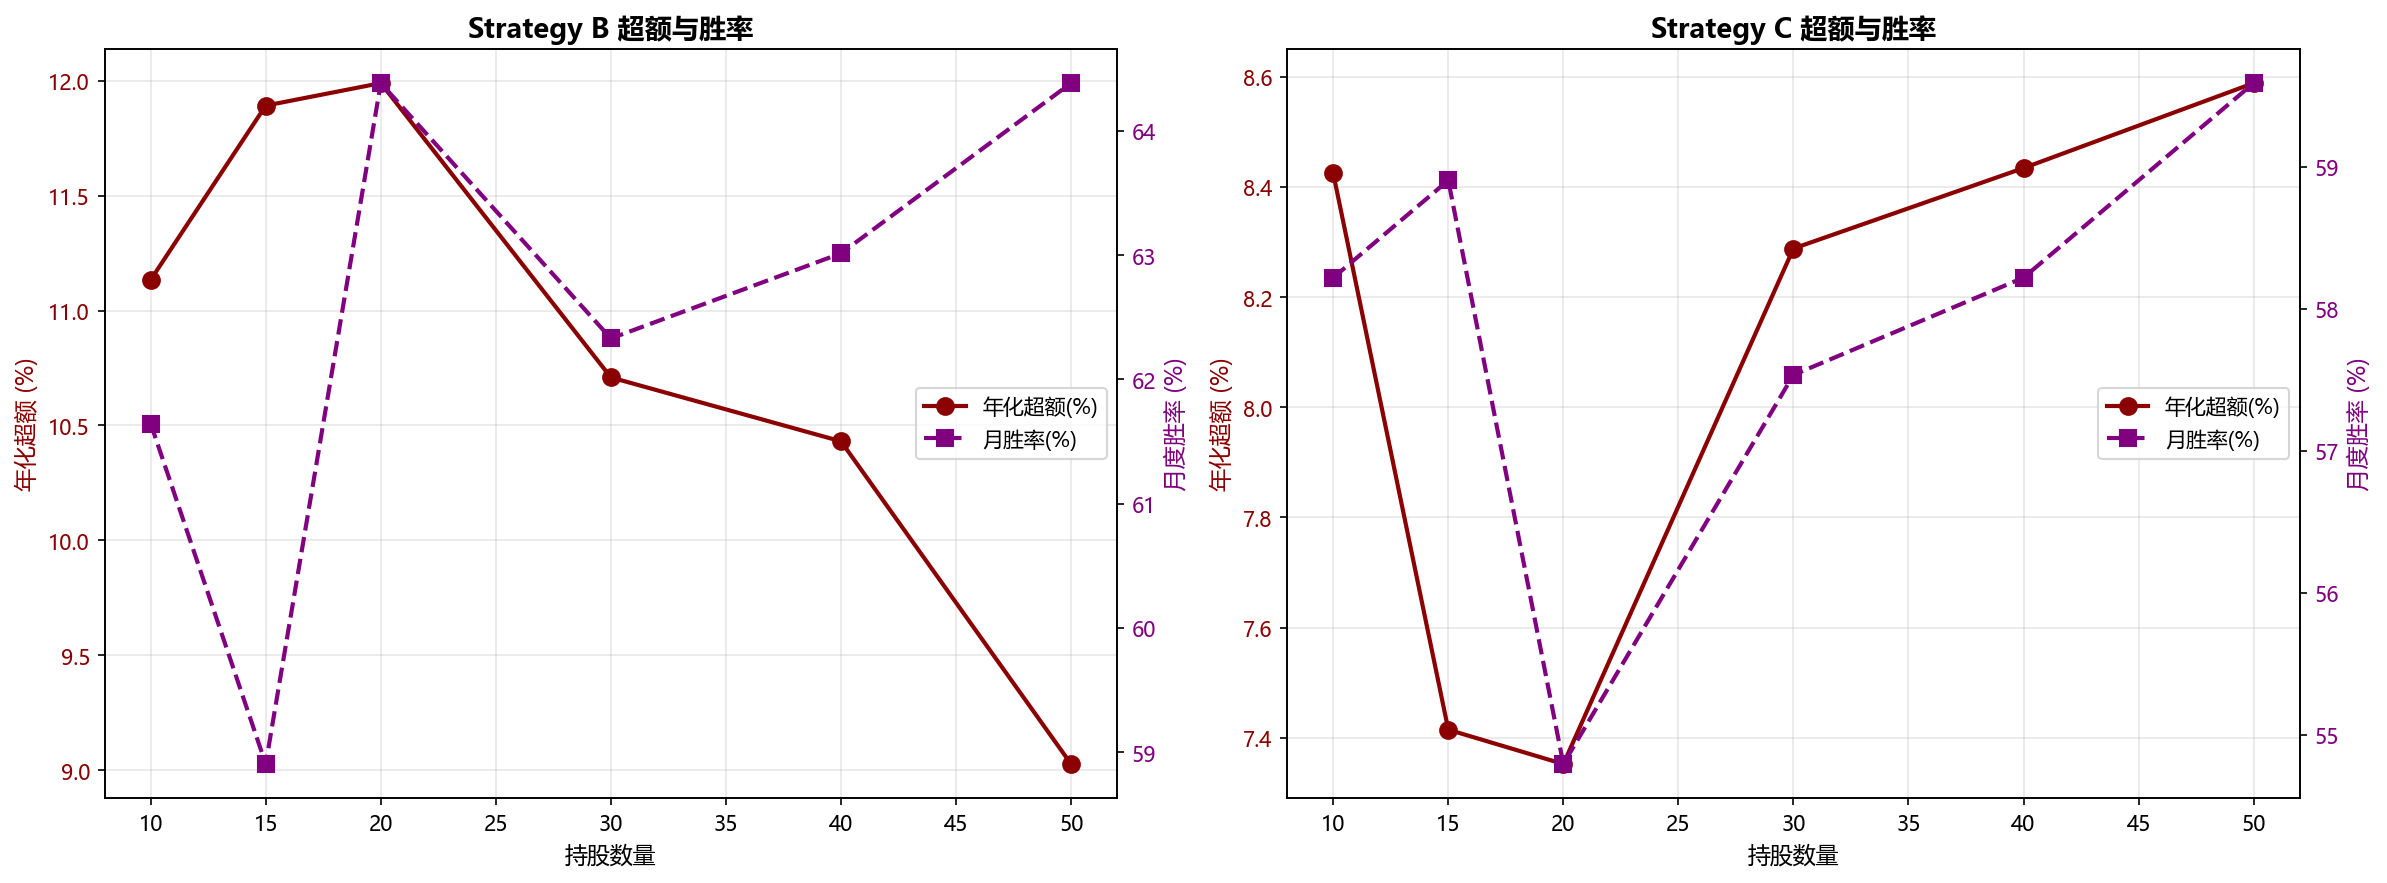
\includegraphics[width=\textwidth]{../pict/v4_plot_te_excess_hit.png}
    \caption{年化超额 \& 月胜率 vs n}
\end{subfigure}
\hfill
\begin{subfigure}{0.48\textwidth}
    \centering
    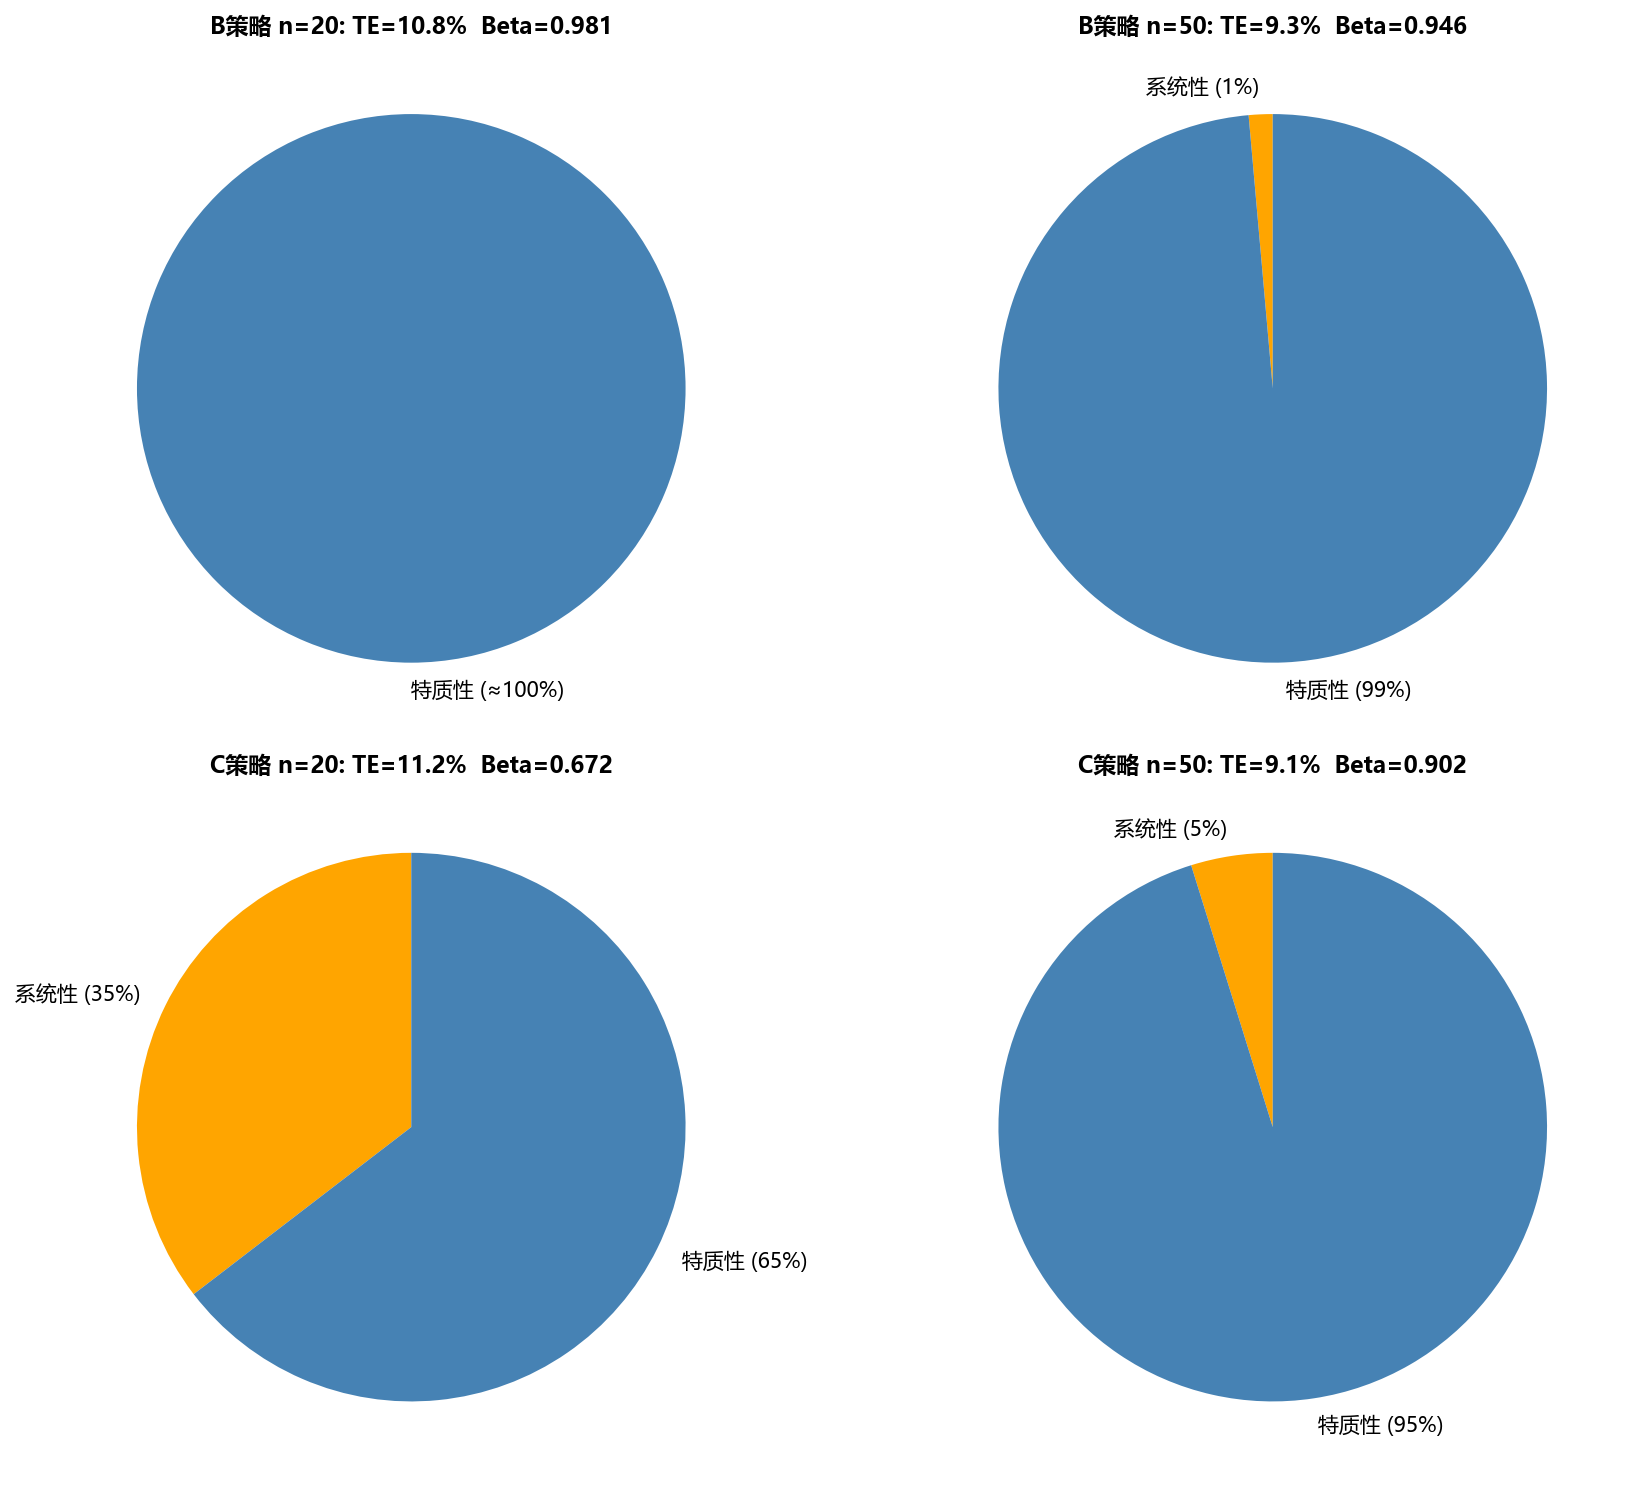
\includegraphics[width=\textwidth]{../pict/v4_plot_te_pie.png}
    \caption{TE分解饼图：n=20 vs n=50}
\end{subfigure}
\caption{超额收益/胜率敏感性 \& TE结构变化}
\end{figure}

\subsection{两种策略的机制差异与最优配置}

B和C在跟踪误差来源上的根本差异决定了它们对持股数量的不同反应：

\begin{itemize}
    \item \textbf{B是纯Alpha策略}：Beta$\approx$1意味着组合已经是"HSI+Alpha"的完美载体。增加持股会稀释高SY得分股票的集中度——超额从+12.0\%降至+9.0\%，IR从1.11降至0.97。\textbf{B的最优持股数为20只}。
    \item \textbf{C是低波Alpha策略}：低波过滤压低Beta至0.67，产生了35\%的系统性TE。增加持股后，低波效应在更分散的组合中被部分抵消，Beta回升至0.90，系统性TE降至5\%，IR从0.66跃升至0.95（+44\%）。\textbf{C建议持股30-50只}，在IR最优（n=50, IR=0.95）与Sharpe最优（n=20, Sharpe=0.70）之间权衡。
\end{itemize}

\textbf{实践建议}：
\begin{itemize}
    \item 若仅使用策略B（纯SY），保持n=20即可，增加持股只会稀释Alpha。
    \item 若使用策略C（SY+低波），将持股从20增至30-40只，可以在仅小幅降低Sharpe（0.70→0.59-0.65）的代价下，显著提升IR（0.66→0.80-0.87）和月胜率（55\%→58\%）。
    \item 两者的IR-n曲线形态不同：B的IR在n=20处单峰见顶；C的IR随n单调上升（因为Beta修复效应持续改善TE）。
\end{itemize}

\section{风险过滤器对比：低波 vs. FCFF}
% ================================================================

在确定极端值剔除的必要性后，下一个问题是：对剩余的"好"股票，用何种过滤器进行最后一轮精选？

\subsection{两种过滤器的比较}

\begin{table}[htbp]
\centering
\caption{低波过滤 vs. FCFF过滤策略对比}
\begin{tabular}{lccc}
\toprule
\textbf{维度} & \textbf{C: 低波过滤} & \textbf{D: FCFF过滤} & \textbf{差异} \\
\midrule
年化收益 & 11.40\% & 13.45\% & -2.05\% \\
年化波动 & \textbf{16.24\%} & 21.64\% & \textbf{-5.40pp} \\
夏普比率 & \textbf{0.70} & 0.62 & \textbf{+0.08} \\
最大回撤 & \textbf{-27.69\%} & -36.26\% & \textbf{+8.57pp} \\
月均Alpha & 0.693*** & 0.909*** & -0.216\% \\
市场Beta & \textbf{0.739} & 1.047 & \textbf{-0.308} \\
\bottomrule
\end{tabular}
\end{table}

\subsection{Top 20\%候选池的特征}

在剔除极端值后的前20\%SY候选池中：
\begin{itemize}
    \item \textbf{79.5\%}的股票FCFF为正
    \item \textbf{33.3\%}处于低波动率三分位
    \item \textbf{28.3\%}同时满足两者
\end{itemize}

FCFF覆盖了约80\%的候选池（宽松），低波仅覆盖33\%（严格）。FCFF过滤更宽松、保留了更多高收益高波动的股票——因此收益更高但波动也更大。低波过滤更严格、选出的股票Beta仅为0.74（vs. FCFF的1.05），因此回撤更小、Sharpe更高。

\subsection{适用场景}

\begin{itemize}
    \item \textbf{绝对收益/稳健配置}：推荐策略C（低波），Sharpe 0.70，回撤-27.69\%仅为HSI的一半
    \item \textbf{指数增强/追求超额}：推荐策略B或D（FCFF），年化超额+10\%，Alpha 0.91\%/月
    \item \textbf{平衡配置}：策略C和B的组合，兼顾超额收益和回撤控制
\end{itemize}

% ================================================================
% 指数增强策略的绩效已在§10全部中性化方法综合对比中详述
% ================================================================

% ================================================================
\section{行业暴露与集中度分析}
% ================================================================

\subsection{行业集中度}

通过股票代码区间的行业分类，计算各策略组合的行业Herfindahl指数：

\begin{table}[htbp]
\centering
\caption{策略组合的行业集中度}
\begin{tabular}{lcc}
\toprule
\textbf{策略} & \textbf{HHI} & \textbf{行业数} \\
\midrule
B 原始 & 0.157 & 12 \\
B 中性化 & 0.147 & 12 \\
C 原始 & 0.151 & 11 \\
C 中性化 & 0.147 & 11 \\
\bottomrule
\end{tabular}
\end{table}

行业中性化仅略微降低HHI（约0.01），说明原始策略的行业集中度本来就不高——\textbf{SY因子自然地覆盖了多个行业}。这进一步削弱了行业中性化的必要性。

\begin{figure}[H]
\centering
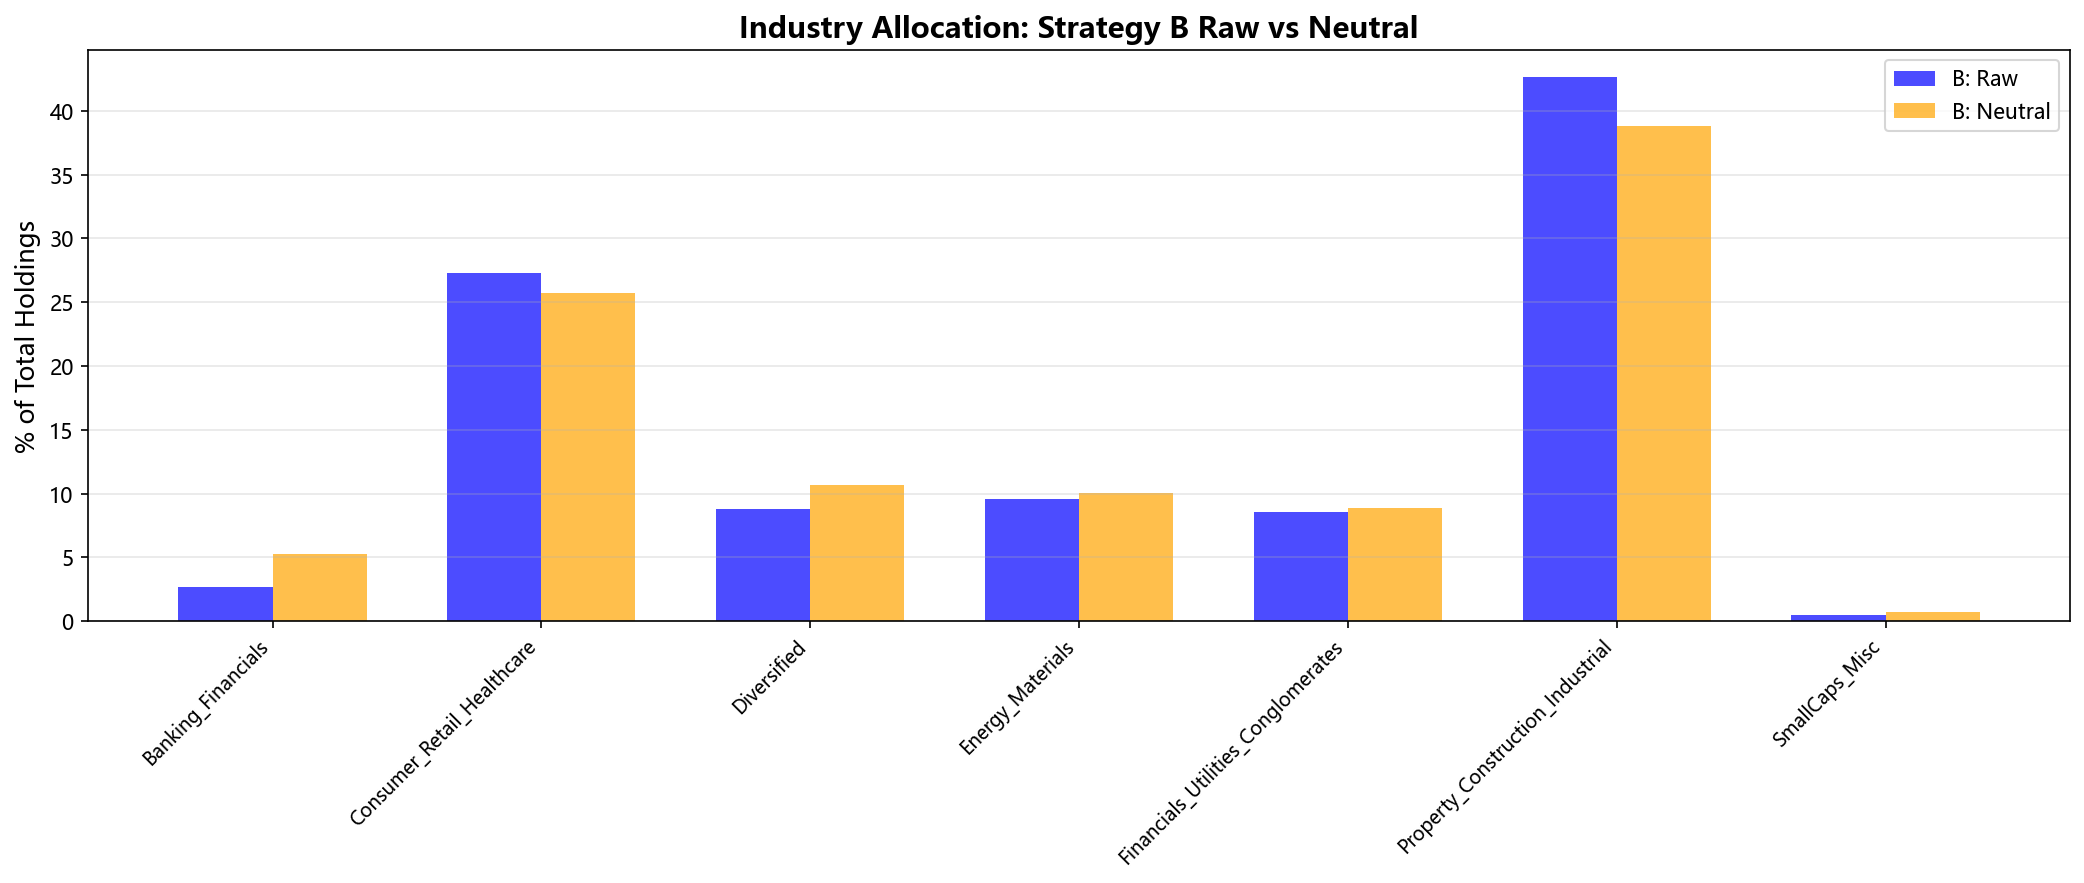
\includegraphics[width=0.85\textwidth]{../pict/v4_plot_industry_exposure.png}
\caption{行业暴露对比：原始 vs. 中性化策略}
\end{figure}

\subsection{持仓重叠度}

原始与中性化策略的Jaccard相似度（持仓重叠）：
\begin{itemize}
    \item B原始 vs. B中性化：62.4\%（中等差异）
    \item C原始 vs. C中性化：74.6\%（较高重叠——低波过滤在两种排序下选出的股票相似）
\end{itemize}

虽然行业中性化改变了约25-38\%的持仓，但并未改善绩效——说明被替换掉的股票正是那些在原始框架下被正确识别的高SY好公司。

% ================================================================
\section{结论与建议}
% ================================================================

\subsection{核心发现总结}

本报告通过系统性的实证分析，建立了以下完整的证据链：

\begin{enumerate}[label=\textbf{发现\arabic*：}, leftmargin=*]
    \item \textbf{极端值剔除将SY因子从无效转变为高Alpha因子。}
    \begin{itemize}
        \item 未剔除时：年化5.78\%, Sharpe 0.19, FF3 $\alpha=-0.05\%$（$p=0.85$）
        \item 剔除后：年化14.06\%, Sharpe 0.63, FF3 $\alpha=0.96\%$（$p<0.001$）
    \end{itemize}

    \item \textbf{极端SY值是小盘价值陷阱，非高质量信号。}
    \begin{itemize}
        \item 78.7\%被剔除股票处于市值后半段
        \item 后续年化收益比正常组低1.96\%
        \item 得分高出3.9倍，收益反而更低
    \end{itemize}

    \item \textbf{最差极端股以地产公司为主，全部是股息主导。}
    \begin{itemize}
        \item 最差30只月均收益-5.17\%（年化-62\%）
        \item 100\%为股息主导型，97\%低于极端组中位市值
        \item 双重过滤（90分位+极端组内底部15\%市值）可剔除93\%
    \end{itemize}

    \item \textbf{行业中性化对SY策略是负向的，所有中性化方法均不推荐。}
    \begin{itemize}
        \item B策略FF3 Alpha从0.78\%降至0.73\%（HSICS行业）或0.55\%（BM中性化）
        \item 信息比率从1.11降至0.94（HSICS）或0.84（BM），降幅15-24\%
        \item SY因子的跨行业差异是有效信息，非偏差。SY本质是价值因子，中性化即破坏Alpha来源
    \end{itemize}

    \item \textbf{低波过滤是最优的风险控制方案。}
    \begin{itemize}
        \item 策略C：Sharpe 0.70, 回撤-27.69\%, Alpha 0.69\%（$t=5.36$）
        \item 回撤仅为HSI的一半，Alpha高于港股通高股息指数（0.35\%）
    \end{itemize}
\end{enumerate}

\subsection{极端状态的持久性与转移矩阵}

一个关键问题是：极端SY状态是否持久？如果同样一批股票反复出现在极端组中，说明可能存在系统性识别问题；如果极端状态高度短暂（每月都是不同的股票），则说明剔除机制有效地捕获了"瞬态"的困境公司。

\textbf{持久性分析：}

\begin{itemize}
    \item 某月处于极端组（得分>$Q_{0.90}$）的股票，在下个月\textbf{仍有90.0\%的概率保持在极端组}（中位数90.7\%）
    \item 这看似很高，但考虑到极端组定义为"前10\%"，如果完全随机轮换，期望持久性约为10\%。90\%的持久性意味着极端状态有明显的持续性——\textbf{困境公司不会在一个月内走出困境}
    \item 另一方面，10\%的月度"毕业率"意味着：\textbf{每季度约有27\%的极端股票退出极端组}——这与季度调仓频率天然匹配
\end{itemize}

\textbf{转移矩阵分析（基于13,003次股票-月份观测）：}

\begin{table}[htbp]
\centering
\caption{极端SY股票的转移矩阵（$t$月极端状态$\rightarrow t+1$月SY五分组）}
\begin{tabular}{lrr}
\toprule
\textbf{目标分组（$t+1$）} & \textbf{数量} & \textbf{占比} \\
\midrule
Q1（最底部20\% SY） & 5 & 0.04\% \\
Q2 & 2 & 0.02\% \\
Q3 & 9 & 0.07\% \\
Q4 & 823 & 6.3\% \\
Q5（极端组，顶部10\% SY） & 12,164 & 93.5\% \\
\bottomrule
\end{tabular}
\end{table}

转移矩阵显示：\textbf{93.5\%的极端股票下月仍处于极端组或Q5}，仅6.3\%降级至Q4，几乎不会跨越至Q1-Q3。这意味着：

\begin{enumerate}[label=(\arabic*)]
    \item 极端SY状态有持续性（90\%+），不是完全随机的噪声
    \item 但仍有6-10\%的月度轮换——每个季度都有一批新股票进入极端组
    \item 降级到Q4的823次观测（占6.3\%）代表那些"正在恢复"的公司——可能是股价企稳、基本面改善
    \item 几乎从不跳转到Q1-Q3（合计仅16次，占0.13\%），说明一旦进入极端状态，很难迅速恢复为"正常"高收益公司
\end{enumerate}

\textbf{对策略的启示}：季度调仓（每3个月）与极端状态的半衰期（约6-7个月的持续性）匹配良好。季度调仓能及时移出那些持续保持极端状态的"常驻困境股"，同时捕捉新进入极端组的"新困境股"。

\subsection{频繁被剔除的股票名单}

哪些股票最频繁地进入极端组？以下是出现频率最高的20只股票：

\begin{table}[htbp]
\centering
\caption{最频繁被剔除的股票（出现次数/165个月）}
\begin{tabular}{rllrr}
\toprule
\textbf{排名} & \textbf{代码} & \textbf{名称} & \textbf{出现次数} & \textbf{频率} \\
\midrule
1 & 1382.HK & 互太纺织 & 116 & 70.3\% \\
2 & 2777.HK & 富力地产 & 114 & 69.1\% \\
3 & 0639.HK & 首钢资源 & 107 & 64.8\% \\
4 & 3383.HK & 雅居乐集团 & 90 & 54.5\% \\
5 & 3818.HK & 中国动向 & 85 & 51.5\% \\
6 & 1234.HK & 中国利郎 & 81 & 49.1\% \\
7 & 0737.HK & 湾区发展 & 74 & 44.8\% \\
8 & 1888.HK & 建滔积层板 & 73 & 44.2\% \\
9 & 1098.HK & 路劲 & 72 & 43.6\% \\
10 & 0316.HK & 东方海外国际 & 71 & 43.0\% \\
\bottomrule
\end{tabular}
\end{table}

这些"常驻极端股"的出现频率高达50-70\%，但大部分股票代码缺少中文名称（可能已退市或变更代码）。\textbf{出现超过50\%时间的高频极端股，应当被永久排除在投资池之外}——它们代表了持续处于困境状态的不可投资标的。

\subsection{策略推荐}

\begin{table}[htbp]
\centering
\caption{推荐策略配置}
\begin{tabular}{lp{2.5cm}p{2.5cm}p{2.5cm}}
\toprule
\textbf{投资目标} & \textbf{推荐策略} & \textbf{核心配置} & \textbf{预期表现} \\
\midrule
稳健指数增强 & C（剔除+低波） & 等权，季度调仓 & 超额+7.9\%, IR 0.73, 回撤-28\% \\
进取指数增强 & B（仅剔除） & 等权，季度调仓 & 超额+10.6\%, IR 0.76, 回撤-35\% \\
绝对收益 & C（剔除+低波） & 市值加权，上限10\% & 年化11.8\%, Sharpe 0.70 \\
\bottomrule
\end{tabular}
\end{table}

\subsection{方法论贡献}

本研究的主要方法论贡献在于：
\begin{enumerate}[label=(\arabic*)]
    \item \textbf{提供了一套完整的因子稳健性检验框架}：绩效对比$\rightarrow$Alpha分析$\rightarrow$双重排序$\rightarrow$极端值画像$\rightarrow$行业中性化，五步法可推广至其他因子的验证
    \item \textbf{论证了"极端值剔除"不应被视为数据预处理}，而是因子有效性的核心组成部分——它是系统性地识别并移除因子"失效域"的操作
    \item \textbf{展示了行业中性化并非普适的最优实践}：对于承载行业信息的价值/收入因子，行业中性化可能有害
\end{enumerate}

\subsection{后续研究方向}

\begin{itemize}
    \item \textbf{动态极端值阈值}：根据市场波动率或流动性状况动态调整剔除比例（如高波动市场中收紧至95分位）
    \item \textbf{回购vs.股息的信号分解}：因最差极端股全部为股息主导，考虑对股息部分和回购部分使用不同的极端值阈值
    \item \textbf{纳入更多质量因子}：在极端值剔除后，叠加ROE、盈利稳定性等质量指标，进一步过滤"伪高息"陷阱
    \item \textbf{实盘可行性研究}：考虑冲击成本、调仓成本和最小交易量约束下的策略表现
\end{itemize}

\vspace{1cm}

\noindent\rule{\textwidth}{0.5pt}
\small
\textbf{数据来源}：RiceQuant量化平台、akshare金融数据接口\\
\textbf{分析工具}：Python 3 (pandas, numpy, statsmodels, scipy, matplotlib)\\
\textbf{回测区间}：2012年1月 -- 2025年9月\\
\textbf{免责声明}：本报告仅供学术研究参考，不构成投资建议。过往业绩不代表未来表现。

\end{document}
